\chapter{ESTADO DEL ARTE}\label{chap:background}
\vskip 3.0ex

% \documentclass statement and preamble
En este capítulo se realiza una revisión del trabajo previo realizado en compresión de grafos, se profundiza sobre las posibles estructuras compactas a utilizar, y se detalla el problema y la solución a utilizar para la detección de cliques maximales.

\section{Compresión de grafos}
El problema de compresión de grafos ha sido abordado de distintas maneras en las últimas décadas. En esta sección se revisan los trabajos más relevantes del área.

\subsection{The WebGraph Framework, \textit{Boldi y Vigna}}
Uno de los primeros trabajos en la materia es \textit{WebGraph} de Boldi y Vigna \cite{boldi2004webgraph}, apuntado a comprimir grafos dirigidos como el grafo de la Web, aprovechando la distribución potencial de las diferencias entre vecinos sucesivos, reflejados en dos características de sus enlaces ordenados por su \textit{URL}, \textbf{localidad} (hipervínculos donde sus \textit{URL} tienen un prefijo en común y si se ordenan lexicográficamente en una lista estarán muy cerca entre ellos) y \textbf{similitud} (los sitios que tienden a estar juntos en esa lista lexicográfica también tienden a tener muchos sucesores en común). Así, codifican las listas de adyacencias basadas en otras listas de adyacencias y cuán similar sean entre ellas.

Primero, cada nodo se numeran los $N$ nodos del grafo de $0$ a $N - 1$, ordenados de manera lexicográfica según sus \textit{URL}. En una primera aproximación, cada nodo tiene asociado su grado de salida (\textit{Outdegree}) y su listado de adyacencia o sucesores asociado $S(x)$. Luego,  aprovechando la localidad  de los nodos en dichas listas, se pueden representar usando las diferencias entre sus nodos, quiere decir si $S(x) = (s_{1}, s_{2}, ..., s_{k})$ es el listado de sucesores del nodo $x$ con $k$ vecinos, se codifica como $(s_{1} - x, s_{2} - s_{1} - 1, ..., s_{k} - s_{k - 1} - 1)$. En la Tabla~\ref{table:webgraph1} se muestran ambos casos, usando listado de sucesores y usando la diferencia. Para evitar tener que lidiar con números negativos, el primer número en esta nueva secuencia se codifica de la siguiente manera:

\begin{align}
	w(x) =  \begin{cases}
					2x & x \geq 0 \\
					2|x| - 1 & x < 0
				\end{cases} 
\end{align}

 \begin{table}[b]
\caption{Representación de Webgraph usando listado de sucesores directo y con brechas.}
\label{table:webgraph1}
\centering
\scriptsize

\begin{tabular}{|l|l|l|l|}
	\toprule
	Nodo & Outd. & Sucesores & Usando brechas \\
	\midrule
	... & ... & ... & ... \\
	15 & 11 & 13, 15, 16, 17, 18, 19, 23, 24, 203, 315, 1034 & 3, 1, 0, 0, 0, 0, 3, 0, 178, 111, 718 \\
	16 & 10 & 15, 16, 17, 22, 23, 24, 315, 316, 317, 3041 & 1, 0, 0, 4, 0, 0, 290, 0, 0, 2723 \\
	17 & 0 &  &  \\
	18 & 5 & 13, 15, 16, 17, 50 & 9, 1, 0, 0, 32 \\
	... & ... & ... & ... \\
\end{tabular}
\end{table} 


Avanzando en el modelo de compresión, cada nodo tiene un entero $r$ llamado referencia, si $r = 0$ la lista no está comprimida usando una referencia, y para $r > 0$ la lista $x$ está definida por la diferencia de la lista $x - r$. Un bitmap llamado \textit{copy list} codifica los sucesores que deben ser copiados a la lista, con un $1$ si el nodo referenciado esta presente en dicha lista o no. Adicionalmente se usa una lista extra para agregar todos los nodos remanentes. Las copy list se codifican en \textit{copy blocks}, donde el primer block es $0$ si la copy list comienza con un $0$. Un bloque se representa por l largo de $0$ o $1$ en la lista menos uno, y el último bloque se omite. En las Tablas \ref{table:webgraph2} y \ref{table:webgraph3} se ilustra un ejemplo para ambos casos.

\begin{table}[t]
\caption{Representación de Webgraph usando copy list.}
\label{table:webgraph2}
\centering
\scriptsize

\begin{tabular}{|l|l|l|l|l|}
	\toprule
	Nodo & Outd. & Ref. & Copy list & Nodos extra \\
	\midrule
	... & ... & ... & ... & ... \\
	15 & 11 & 0 &  & 13, 15, 16, 17, 18, 19, 23, 24, 203, 315, 1034 \\
	16 & 10 & 1 & 01110011010 & 22, 316, 317, 3041 \\
	17 & 0 &  &  &  \\
	18 & 5 & 3 & 11110000000 & 50 \\
	... & ... & ... & ... & ... \\
\end{tabular}
\end{table} 
 

\begin{table}%[t]
\caption{Representación de Webgraph usando copy blocks.}
\label{table:webgraph3}
\centering
\scriptsize

\begin{tabular}{|l|l|l|l|l|l|}
	\toprule
	Nodo & Outd. & Ref. & \# blocks & Copy blocks & Nodos extra \\
	\midrule
	... & ... & ... & ... & ... & ... \\
	15 & 11 & 0 &  &  & 13, 15, 16, 17, 18, 19, 23, 24, 203, 315, 1034 \\
	16 & 10 & 1 & 7 & 0, 0, 2, 1, 1, 0, 0 & 22, 316, 317, 3041 \\
	17 & 0 &  &  &  & \\
	18 & 5 & 3 & 1 & 4 & 50 \\
	... & ... & ... & ... & ... & ... \\
\end{tabular}
\end{table}


Como se puede apreciar de los ejemplos, la consecutividad es frecuente en el listado de nodos extra. Este hecho se puede aprovechar en un paso previo a la compresión por brecha, aislando las subsecuencias correspondientes a intervalos de enteros. Sólo los intervalos de largo no menor a un cierto umbral $L_{min}$ son considerados. Entonces, cada listado de nodos extra se comprime de la siguiente manera:

\begin{itemize}
	\item Un listado de intervalos de enteros. Se representa cada intervalo por su valor extremo izquierdo y su largo. Su valor extremo izquierdo se comprime usando la diferencia entre si mismo y el previo extremo derecho menos dos, ya que debe haber al menos un entero entre el final de un intervalo y el inicio del siguiente. Al largo del intervalo se le resta el umbral $L_{min}$.
	\item Una lista de nodos residuales, los que no son parte de los intervalos anteriores, comprimida usando la diferencia.
\end{itemize}

\begin{table}%[b]
\caption{Representación de Webgraph usando intervalos, con umbral $L_{min} = 2$.}
\label{table:webgraph4}
\centering
\scriptsize

\begin{tabular}{|l|l|l|l|l|l|l|l|l|}
	\toprule
	Nodo & Outd. & Ref. & \# blocks & Copy blocks & \# intervalos & Ext. izq. & Largo & Residuales \\
	\midrule
	... & ... & ... & ... & ... & ...  & ...  & ...  & ... \\
	15 & 11 & 0 &  &  & 2 & 0, 2 & 3, 0 & 5, 189, 111, 718 \\
	16 & 10 & 1 & 7 & 0, 0, 2, 1, 1, 0, 0 & 1 & 600 & 0 & 12, 3018 \\
	17 & 0 &  &  &  &  &  &  & \\
	18 & 5 & 3 & 1 & 4 & 0 &  &  & 50 \\
	... & ... & ... & ... & ... & ...  & ...  & ...  & ... \\
\end{tabular}
\end{table} 


Finalmente, en la Tabla~\ref{table:webgraph4} se puede apreciar la representación comprimida resultante, con un umbral $L_{min} = 2$. 

En un trabajo posterior Boldi et. al. \cite{boldi2009permuting}, usando la matriz de adyacencia y basados en aplicar permutaciones a sus filas, logran reordenar y generar una nueva matriz donde las filas, si son similares (contienen 1s en posiciones muy comunes), deben ser consecutivas o en una vecindad acotada. En otro trabajo propusieron un nuevo algoritmo llamado \textit{Layered Label Propagation} \cite{boldi2011layered} (propagación de etiquetas por capas). Su objetivo era poder ocupar las técnicas desarrolladas anteriormente para grafos de redes sociales, donde los vértices no pueden ser ordenados de manera lexicográfica. Usando la matriz de adyacencia, junto con descomponer en tareas el re-ordenamiento de la matriz y aprovechar los procesadores multi-core, logran muy buenos resultados.

Francisco, Gagie, Ladra y Navarro \cite{francisco2018exploiting} estudian cómo potenciar el cálculo del producto de matrices con vectores de una manera eficiente, por ejemplo para PageRank\cite{page1999pagerank}.  Además, demuestran que se puede aprovechar el formato de algunos esquemas de compresión, en particular el de Boldi y Vigna, para hacer el cálculo en un tiempo proporcional al tamaño de la matriz comprimida.
 %discute algunos algoritmos de compresión de grafos que permiten explotar en forma amigable la computación de matrices. En particular, muestran como el formato de WebGraph  que además son usados en algoritmos de ranking como PageRank \cite{page1999pagerank}.


\subsection{BFS, \textit{Apostolico y Drovandi}}
Otra alternativa de compresión bastante competitiva, también para grafos dirigidos, es la que presentan Apostolico y Drovandi \cite{apostolico2009graph}, basado en la topología del grafo de la Web en vez de las \textit{URL} subyacentes. En vez de asignarle índices a los nodos según el orden lexicográfico de sus \textit{URL}, realizan un recorrido por \textit{breath-first} o búsqueda en anchura del grafo, numerando cada nodo según el orden en que se expanden. Este proceso y su compresión inducida lo llaman \textit{Fase 1}, y la compresión de las aristas remanentes como \textit{Fase 2}.

En la Fase 1, al expandir un nodo $v_{i} \in V$ se le asignan índices enteros consecutivos a sus $k_{i}$ vecinos, y se guarda el valor $k_{i}$. Cuando el recorrido del grafo se completa, todas las aristas que pertenecen al árbol de búsqueda por anchura quedan codificadas en la secuencia $\{k_{1}, k_{2}, ..., k_{|V|}\}$ llamada \textit{traversal list} (lista de recorrido). En la Figura~\ref{fig:bfs1} se presenta un ejemplo para la Fase 1, donde en (a) se presenta el orden de los nodos asignados por BFS, y en (b) las aristas restantes junto con el listado de recorrido.

\begin{figure}%[b]
    	\centering
    	\begin{minipage}{0.45\textwidth}
    		\centering
    		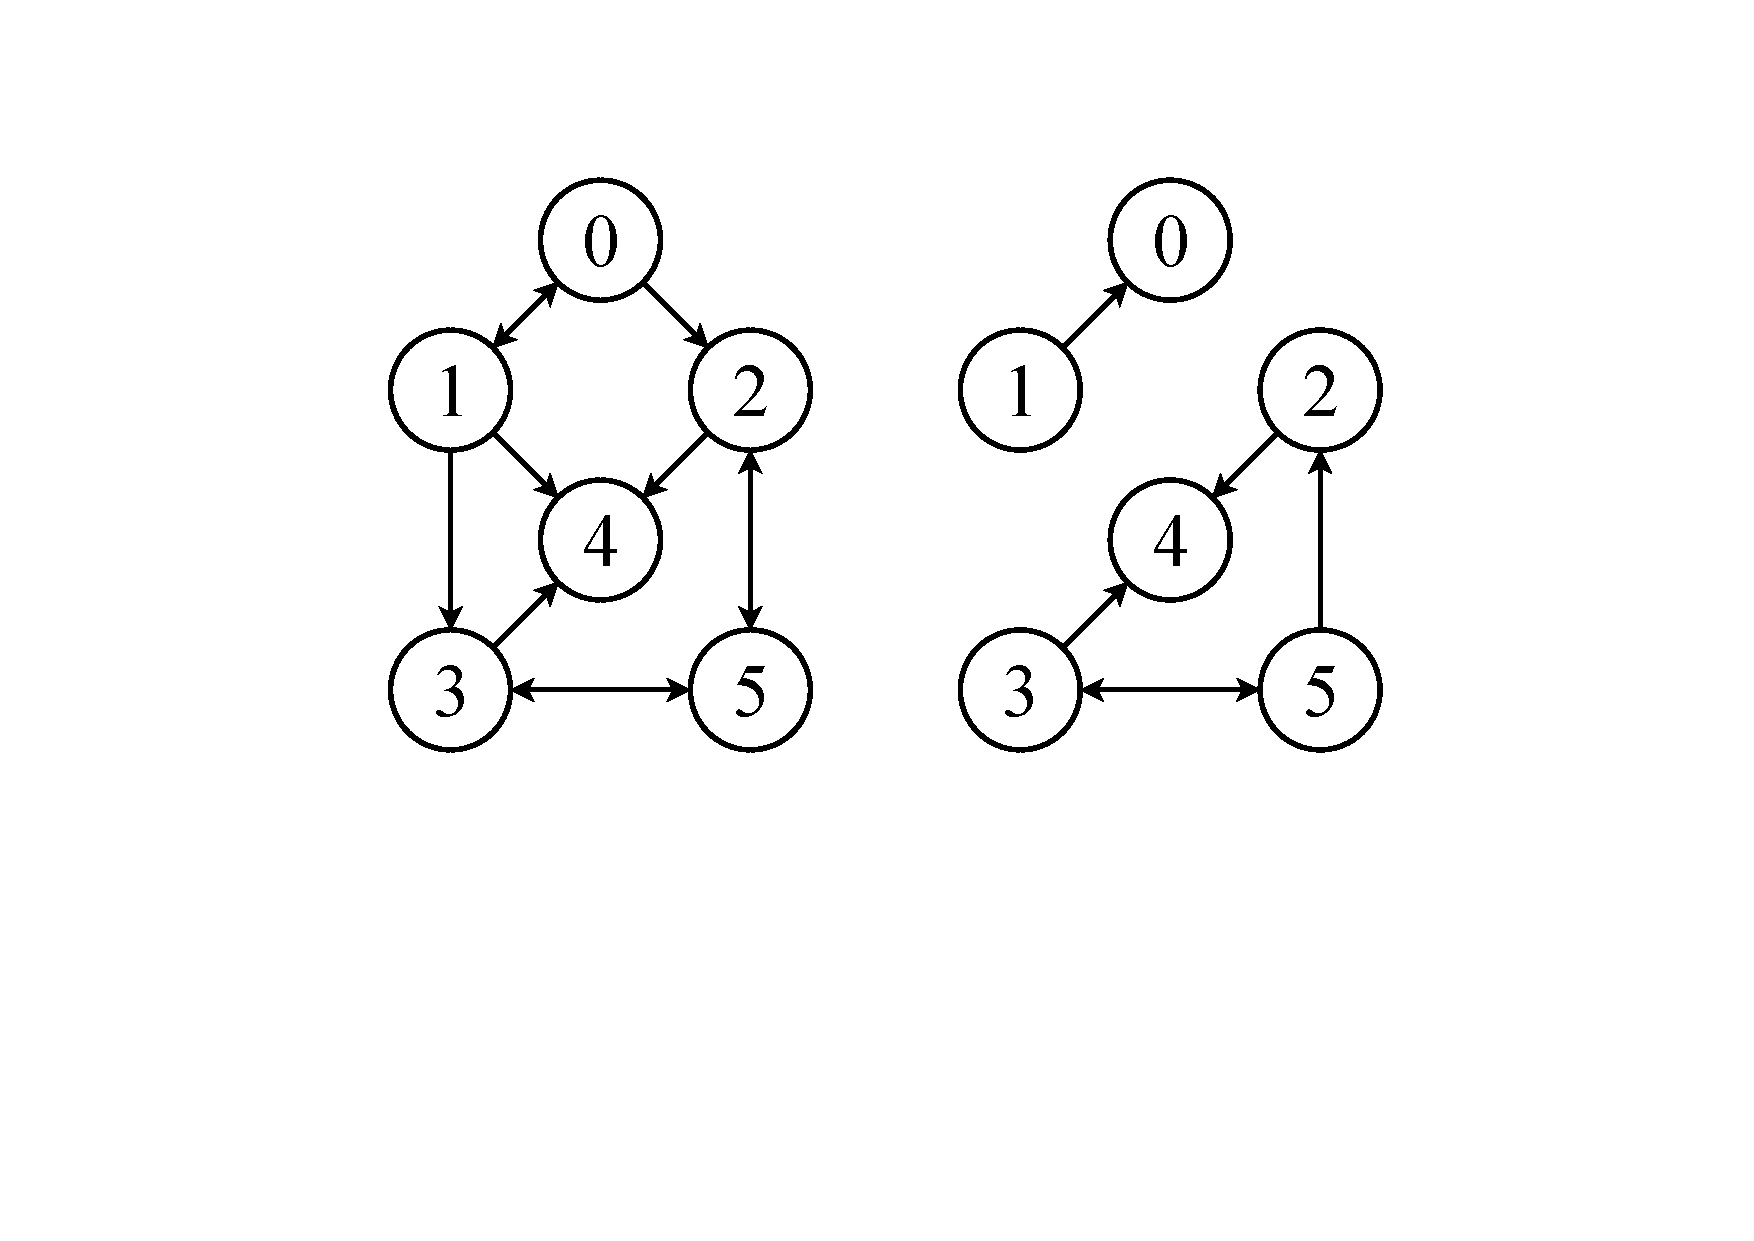
\includegraphics[scale=.3, clip, trim=180 230 440 80 ]{img/arte/graphs-BFS-F1.pdf}
    		
    		(a)
    	\end{minipage}
    	\begin{minipage}{0.45\textwidth}
    		\centering
    		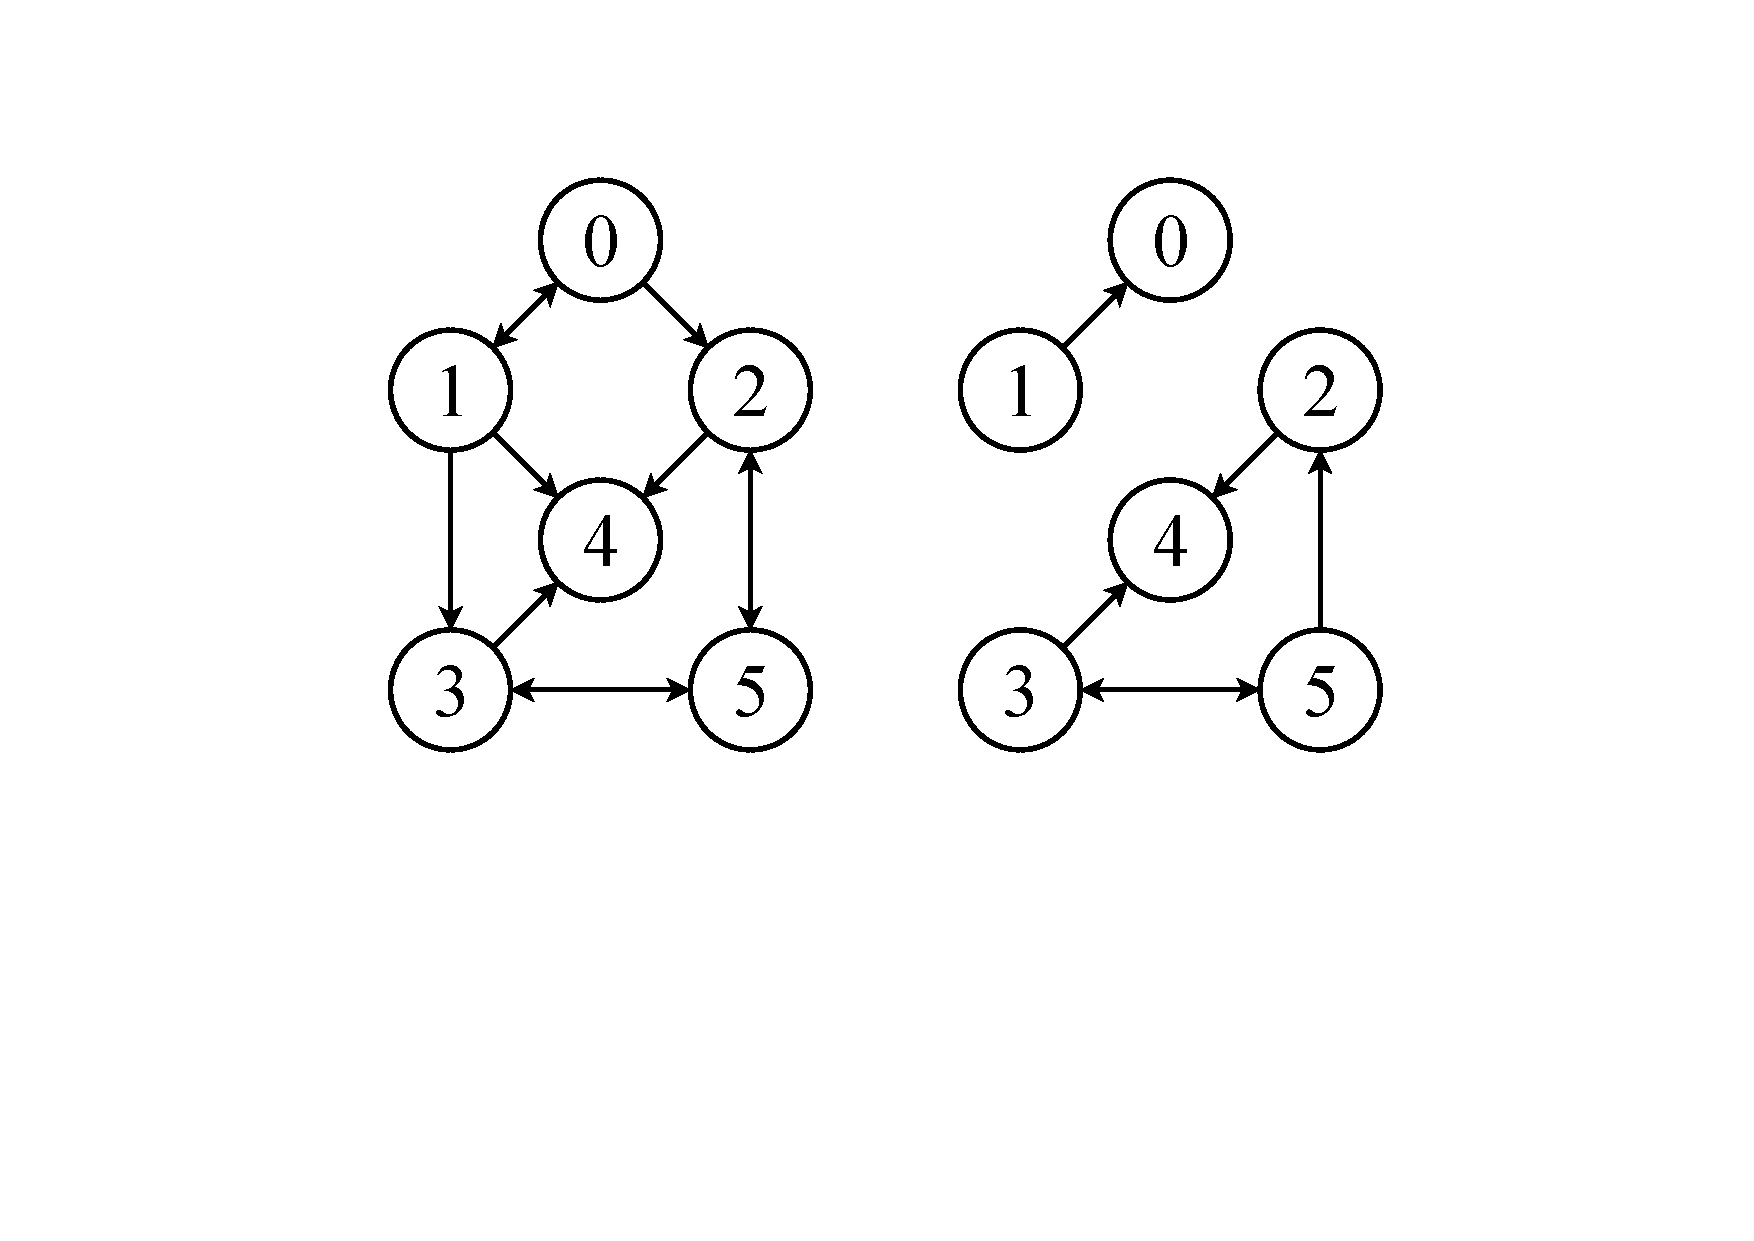
\includegraphics[scale=.3, clip, trim=450 230 170 80]{img/arte/graphs-BFS-F1.pdf}
    		
    		$T = \{2, 2, 1, 0, 0, 0\}$
    		
    		(b)
    	\end{minipage}

    \caption{Ejemplo de Fase 1 de BFS. (a) Índices asignados a los nodos. (b) Aristas restantes después de BFS, junto listado de recorrido $T$.}
    \label{fig:bfs1}
\end{figure}


Luego comprimen por separado trozos consecutivos de $l$ nodos, siendo $l$ un valor específico que define el nivel de compresión. Cada trozo comprimido $C$, conformado por los nodos $v_{i}, v_{i + 1}, ..., v_{i + l - 1}$, lleva prefijado la secuencia $\{k_{i}, k_{i + 1}, ..., k_{i + l - 1}\}$.

En la Fase 2, codifican la lista de adyacencia $A_{i}$ de cada nodo $v_{i} \in V$ de un trozo $C$ en orden creciente. Cada lista codificada consiste en la diferencia entre elementos adyacentes en la lista y un indicador tipo del set $\{\alpha, \beta, \chi, \phi\}$. Con $A_{i}^{j}$ indicando el elemento $j$ de la lista $A_{i}$, distinguen tres casos:

\begin{enumerate}
	\item $A_{i - 1}^{j} \leq A_{i}^{j - 1} < A_{i}^{j}$: el código es $\phi \cdot (A_{i}^{j} - A_{i}^{j - 1} - 1)$.
	\item $A_{i}^{j - 1} < A_{i - 1}^{j} \leq A_{i}^{j}$: el código es $\beta \cdot (A_{i}^{j} - A_{i - 1}^{j})$.
	\item $A_{i}^{j - 1} < A_{i}^{j} < A_{i - 1}^{j}$: se subdivide en dos subcasos:
	\begin{enumerate}
		\item Si $A_{i}^{j} - A_{i}^{j - 1} - 1 \leq A_{i - 1}^{j} - A_{i}^{j} - 1$: el código es $\alpha \cdot (A_{i}^{j} - A_{i}^{j - 1} - 1)$.
		\item De otro modo: el código es $\chi \cdot (A_{i - 1}^{j} - A_{i}^{j} - 1)$.
	\end{enumerate}
\end{enumerate}

Los tipo $\alpha$ y $\phi$ codifican la diferencia con respecto al elemento previo de la lista ($A_{i}^{j - 1}$), mientras $\beta$ y $\chi$ con respecto al elemento en la misma posición de la lista de adyacencia del nodo previo ($A_{i - 1}^{j}$). Cuando $A_{i - 1}^{j}$ no existe se reemplaza por $A_{k}^{j}$, donde $k (k < i - 1 \wedge v_{k} \in C)$ es el índice más cercano a $i$ para cual el grado de $v_{k}$ no es menor que $j$, o por un código tipo $\phi$ en caso que un nodo así no exista.

En la Tabla~\ref{table:bfs-adjacency} se ilustra un ejemplo de listado de adyacencia, y en la Tabla~\ref{table:bfs-coded} su codificación basada en los casos ya mencionados.

 \begin{table}%[b]
\caption{Lista de adyacencia para BFS, con $v_{i}$ siendo el primer nodo de un trozo.}
\label{table:bfs-adjacency}
\centering
\footnotesize

\begin{tabular}{|l|l|l|}
	\toprule
	Nodo & Grado & Adyacentes \\
	\midrule
	... & ... & ... \\
	i & 8 & 13, 15, 16, 17, 20, 21, 23, 24 \\
	i + 1 & 9 & 13, 15, 16, 17, 19, 20, 25, 31, 32 \\
	i + 2 & 0 &  \\
	i + 3 & 2 & 15, 16 \\
	... & ... & ... \\
\end{tabular}
\end{table} 


 \begin{table}%[b]
\caption{Codificación BFS del listado de adyacencia en la Tabla~\ref{table:bfs-adjacency}.}
\label{table:bfs-coded}
\centering
\footnotesize

\begin{tabular}{|l|l|l|}
	\toprule
	Nodo & Grado & Adyacentes \\
	\midrule
	... & ... & ... \\
	i & 8 & $\phi13$, $\phi1$, $\phi0$, $\phi0$, $\phi2$, $\phi0$, $\phi1$, $\phi0$ \\
	i + 1 & 9 & $\beta0$, $\beta0$, $\beta0$, $\beta0$, $\chi0$, $\alpha0$, $\beta2$, $\phi5$, $\phi0$ \\
	i + 2 & 0 &  \\
	i + 3 & 2 & $\beta2$, $\alpha0$ \\
	... & ... & ... \\
\end{tabular}
\end{table} 


Luego, aprovechan distintos tipos de redundancias en los listados de adyacencia, como se puede ver en la Tabla~\ref{table:bfs-exploting}, distinguiendo cuatro casos:

\begin{enumerate}
	\item Un conjunto de líneas idénticas (ver bloque ancho amarillo en la Tabla~\ref{table:bfs-exploting}) se codifican asignando un multiplicador a la primera línea de la secuencia.
	\item Los intervalos con grado constante de nodos (ver bloque consecutivo de 9s en la Tabla~\ref{table:bfs-exploting}), se codifican por su diferencia.
	\item Una secuencia de largo $\mathcal{L}_{min}$ de elementos idénticos (ver el bloque de $\phi1$s en la Tabla~\ref{table:bfs-exploting}), se codifica por su largo.
	\item Un bloque de filas idénticas (ver gran bloque azul en la Tabla~\ref{table:bfs-exploting}) que superen un umbral $\mathcal{A}_{min}$, se codifica por su largo.
\end{enumerate}

 \begin{table}%[b]
\caption{Ejemplo de redundancias a explotar en listado de adyacencia de BFS.}
\label{table:bfs-exploting}
\centering
\footnotesize

\begin{tabular}{|l|llllllllll|}
	\toprule
	Grado & \multicolumn{9}{l}{Adyacentes} & \\
	\midrule
	\cellcolor{blanco} ... & \multicolumn{9}{l}{\cellcolor{blanco} ...} & \\
	\cellcolor{blanco} 0 & \multicolumn{9}{l}{} & \\
	\cellcolor{rojo} 9 & \cellcolor{blanco} $\beta1,$ & \cellcolor{cafe} $\phi1,$ & \cellcolor{cafe} $\phi1,$ & \cellcolor{cafe} $\phi1,$ & \cellcolor{blanco} $\phi0,$ & \cellcolor{blanco} $\phi1,$ & \cellcolor{blanco} $\phi1,$ & \cellcolor{blanco} $\phi1,$ & \cellcolor{blanco} $\phi1,$ & \\
    \cellcolor{rojo} 9 & \cellcolor{azul} $\beta0,$ & \cellcolor{azul} $\beta1,$ & \cellcolor{azul} $\beta0,$ & \cellcolor{azul} $\beta0,$ & \cellcolor{azul} $\beta0,$ & \cellcolor{azul} $\beta0,$ & \cellcolor{azul} $\beta0,$ & \cellcolor{azul} $\beta0,$ & \cellcolor{blanco} $\beta2,$ & \\
    \cellcolor{blanco} 10 &  \cellcolor{azul} $\beta0,$ & \cellcolor{azul} $\beta1,$ & \cellcolor{azul} $\beta0,$ & \cellcolor{azul} $\beta0,$ & \cellcolor{azul} $\beta0,$ & \cellcolor{azul} $\beta0,$ & \cellcolor{azul} $\beta0,$ & \cellcolor{azul} $\beta0,$  & \cellcolor{blanco} $\beta1,$ & \cellcolor{blanco} $\phi903$ \\
    \cellcolor{blanco} 10 &  \cellcolor{azul} $\beta0,$ & \cellcolor{azul} $\beta1,$ & \cellcolor{azul} $\beta0,$ & \cellcolor{azul} $\beta0,$ & \cellcolor{azul} $\beta0,$ & \cellcolor{azul} $\beta0,$ & \cellcolor{azul} $\beta0,$ & \cellcolor{azul} $\beta0,$  & \cellcolor{blanco} $\beta223,$ & \cellcolor{blanco} $\phi900$ \\
    \cellcolor{blanco} 10 &  \cellcolor{azul} $\beta0,$ & \cellcolor{azul} $\beta1,$ & \cellcolor{azul} $\beta0,$ & \cellcolor{azul} $\beta0,$ & \cellcolor{azul} $\beta0,$ & \cellcolor{azul} $\beta0,$ & \cellcolor{azul} $\beta0,$ & \cellcolor{azul} $\beta0,$  & \cellcolor{blanco} $\beta1,$ & \cellcolor{blanco} $\alpha0$ \\
    \cellcolor{amarillo} 10 & \cellcolor{verde} $\beta0,$ & \cellcolor{verde} $\beta1,$ & \cellcolor{verde} $\beta0,$ & \cellcolor{verde} $\beta0,$ & \cellcolor{verde} $\beta0,$ & \cellcolor{verde} $\beta0,$ & \cellcolor{verde} $\beta0,$ & \cellcolor{verde} $\beta0,$ & \cellcolor{amarillo} $\beta1,$ & \cellcolor{amarillo} $\beta0$ \\
    \cellcolor{amarillo} 10 & \cellcolor{verde} $\beta0,$ & \cellcolor{verde} $\beta1,$ & \cellcolor{verde} $\beta0,$ & \cellcolor{verde} $\beta0,$ & \cellcolor{verde} $\beta0,$ & \cellcolor{verde} $\beta0,$ & \cellcolor{verde} $\beta0,$ & \cellcolor{verde} $\beta0,$ & \cellcolor{amarillo} $\beta1,$ & \cellcolor{amarillo} $\beta0$ \\
    \cellcolor{amarillo} 10 & \cellcolor{verde} $\beta0,$ & \cellcolor{verde} $\beta1,$ & \cellcolor{verde} $\beta0,$ & \cellcolor{verde} $\beta0,$ & \cellcolor{verde} $\beta0,$ & \cellcolor{verde} $\beta0,$ & \cellcolor{verde} $\beta0,$ & \cellcolor{verde} $\beta0,$ & \cellcolor{amarillo} $\beta1,$ & \cellcolor{amarillo} $\beta0$ \\
    \cellcolor{amarillo} 10 & \cellcolor{verde} $\beta0,$ & \cellcolor{verde} $\beta1,$ & \cellcolor{verde} $\beta0,$ & \cellcolor{verde} $\beta0,$ & \cellcolor{verde} $\beta0,$ & \cellcolor{verde} $\beta0,$ & \cellcolor{verde} $\beta0,$ & \cellcolor{verde} $\beta0,$ & \cellcolor{amarillo} $\beta1,$ & \cellcolor{amarillo} $\beta0$ \\
    \cellcolor{blanco} 10 &  \cellcolor{azul} $\beta0,$ & \cellcolor{azul} $\beta1,$ & \cellcolor{azul} $\beta0,$ & \cellcolor{azul} $\beta0,$ & \cellcolor{azul} $\beta0,$ & \cellcolor{azul} $\beta0,$ & \cellcolor{azul} $\beta0,$ & \cellcolor{azul} $\beta0,$  & \cellcolor{blanco} $\alpha76,$ & \cellcolor{blanco} $\alpha232$ \\
    \cellcolor{blanco} 9 &  \cellcolor{azul} $\beta0,$ & \cellcolor{azul} $\beta1,$ & \cellcolor{azul} $\beta0,$ & \cellcolor{azul} $\beta0,$ & \cellcolor{azul} $\beta0,$ & \cellcolor{azul} $\beta0,$ & \cellcolor{azul} $\beta0,$ & \cellcolor{azul} $\beta0,$  & \cellcolor{blanco} $\beta0$ & \\
	\cellcolor{blanco} ... & \multicolumn{9}{l}{\cellcolor{blanco} ...} & \\
\end{tabular}
\end{table} 


Para ello introducen un nuevo símbolo $\Sigma$, seguido de un indicador $\Sigma_{F}$ toma valor 2 si la redundancia es de tipo 3, 3 si es de tipo 4, o 1 si son ambas. Dependiendo de la redundancia a codificar, el código se expresa como `$tipo\:\Sigma\:\Sigma_{F}\:gap\:l$'  o `$tipo\:\Sigma\:\Sigma_{F}\:gap\:l\:w\:h$', siendo $tipo$ uno de los símbolos del set $\{\alpha, \beta, \chi, \phi\}$, $gap$ un entero indicando la diferencia, $l$ la cantidad de elementos idénticos en la misma línea, $w$ y $h$ el ancho y alto de las columnas y filas idénticas. En la Tabla~\ref{table:bfs-exploted} se ilustra esta codificación para el caso ejemplo de la Tabla~\ref{table:bfs-exploting}.

 \begin{table}%[b]
\caption{Ejemplo de redundancias codificadas de BFS para la Tabla~\ref{table:bfs-exploting}.}
\label{table:bfs-exploted}
\centering
\footnotesize

\begin{tabular}{|l|l|llll|}
	\toprule
	Líneas & Grado & \multicolumn{3}{l}{Enlaces} &  \\
	\midrule
	... & ... & ... & & &  \\
	0 & 0 & & & & \\
	0 & 9 & $\beta7$, & $\phi\:\Sigma\:2\:1\:1$, & $\phi0$, & $\phi\:\Sigma\:2\:1\:2$ \\
	0 & 0 & $\beta\:\Sigma\:3\:0\:7\:5$, & $\beta1$, & $\beta\:\Sigma\:2\:0\:4$, & $\beta2$ \\
	0 & 1 & $\beta1$, & $\phi903$ & & \\
	0 & 0 & $\beta223$, & $\phi900$ & & \\
	0 & 0 & $\beta1$, & $\alpha0$ & & \\
	3 & 0 & $\beta1$, & $\beta0$ & & \\
	0 & 0 & $\alpha76$, & $\alpha232$ & & \\
	0 & -1 & $\beta0$ & & & \\
	... & ... & ... & & &  \\
\end{tabular}
\end{table} 


Finalmente, usan códigos Huffman para codificar $\alpha, \beta, \chi, \phi$, y proponen una nueva codificación $\pi$ para cifrar diferencias, $\Sigma$, y otros enteros.

\textcolor{red}{¿Es muy extendida esta explicación? Quizás podría detallar el método un poco menos.}


\subsection{Using Re-Pair, \textit{Claude y Navarro}}
%Claude y Navarro \cite{claude2010fast} proponen buscar los pares de arcos vecinos más frecuentes y reemplazarlos por nuevos símbolos en forma iterativa hasta que se cumpla un umbral, representando el grafo y el diccionario de símbolos en forma comprimida. En esta propuesta, un \textit{digram} consiste en un par de hipervínculos. Para lograr esta representación, los autores deben encontrar digrams con un número máximo de ocurrencias que no se sobrepongan (que no tengan arcos en común). Encontrar estas ocurrencias es un problema conocido como \textit{maximum matching problem} y es caro computacionalmente ($O(|V|^2\times |E|)$). Independiente de eso y al igual que k2tree, la estructura que proponen mejora con los algoritmos para ordenar los nodos en el grafo, y consiguen mejores resultados en grafos RDF con orden BFS.
El trabajo de Claude y Navarro \cite{claude2010fast} propone usar Re-Pair \cite{larsson2000off}, un método de compresión basado en gramática, para comprimir el grafo de la Web. Re-Pair consiste en buscar el par de símbolos más frecuente en una secuencia y reemplazar cada ocurrencia por un nuevo símbolo, el cual se añade a un diccionario como nueva regla. En la Tabla~\ref{table:repair} se muestra un ejemplo simple de Re-Pair, donde las reglas conforman el diccionario para descomprimir la secuencia.

 \begin{table}%[b]
\caption{Ejemplo de Re-Pair. Las reglas en la tabla conforman el diccionario asociado a la compresión.}
\label{table:repair}
\centering
\small

\begin{tabular}{|l|l|}
	\toprule
	Reglas & String \\
	\midrule
	 & $singing.do.wah.diddy.diddy.dum.diddy.do$ \\
	$A \rightarrow .d$ & $singingAo.wahAiddyAiddyAumAiddyAo$ \\
	$B \rightarrow dd$ & $singingAo.wahAiByAiByAumAiByAo$ \\
	$C \rightarrow Ai$ & $singingAo.wahCByCByAumCByAo$ \\
	$D \rightarrow By$ & $singingAo.wahCDCDAumCDAo$ \\
	$E \rightarrow CD$ & $singingAo.wahEEAumEAo$ \\
	$F \rightarrow in$ & $sFgFgAo.wahEEAumEAo$ \\
	$G \rightarrow Ao$ & $sFgFgG.wahEEAumEG$ \\
	$H \rightarrow Fg$ & $sHHG.wahEEAumEG$ \\
	\bottomrule
\end{tabular}
\end{table} 


Claude y Navarro \cite{claude2010fast} aplican esta idea a los listados de adyacencia de un grafo dirigido. Si $V = \{v_{1}, v_{1}, ..., v_{n}\}$ es el listado de $n$ nodos del grafo $G$, $adj(v_{i}) = \{v_{i,1}, v_{i,2},... , v_{i,a_{i}}\}$ el listado de $a_{i}$ nodos adyacentes a $v_{i}$, y $\overline{v_{i}}$ una alternativa de notación para el nodo $v_{i}$, proponen concatenar todos los listados de adyacencia con la siguiente notación:

\begin{equation} \label{eq:RepairGrafo}
	T = T(G) = \overline{v_{1}} \; v_{1,1}, v_{1,2}, ..., v_{1,a_{1}}, \overline{v_{2}} \; v_{2,1}, v_{2,2}, ..., v_{2,a_{2}}, ..., \overline{v_{n}} \; v_{n,1}, v_{n,2}, ..., v_{n,a_{n}}
\end{equation}

\noindent donde se debe cumplir con $v_{i,j} < v_{i, j+1}$ para cualquier $1 \leq i \leq n$ y $1 \leq j \leq a_{i}$. Esto significa que cada lista de adyacencia concatenada debe partir con su nodo referencia, y todos los nodos de ella deben estar ordenados de menor a mayor. Luego se van reemplazando recursivamente, sin incluir los nodos de referencia, los pares de símbolos consecutivos más frecuentes por uno nuevo, hasta que no sea conveniente, y cada reemplazo se guarda como regla. 

Finalmente, se eliminan los nodos de referencia con el cuidado de codificar en dos bitmaps: En $B1$ si tienen nodos adyacentes, y en $B2$ la ubicación de dichos nodos en el arreglo final. En la Figura~\ref{fig:repairCN} se ilustra un ejemplo, donde en (a) se tiene el grafo de ejemplo, en (b) la concatenación $T(G)$ de todos los listados de adyacencia ordenados de menor a mayor, los reemplazos necesarios para su compresión y el arreglo resultante, y en (c) los bitmaps indicadores de los nodos de referencia. Se debe notar que la notación alternativa $\overline{v_{i}}$ se reemplaza por $-v_{i}$ en el arreglo. También presentan otras mejoras, como usar diferencias para codificar los listados de adyacencia o reordenar los nodos para aprovechar mejor Re-Pair.

\begin{figure}%[b]
    	\centering
    	\begin{minipage}{1\textwidth}
    		\begin{minipage}{.6\textwidth}
    			\centering
    			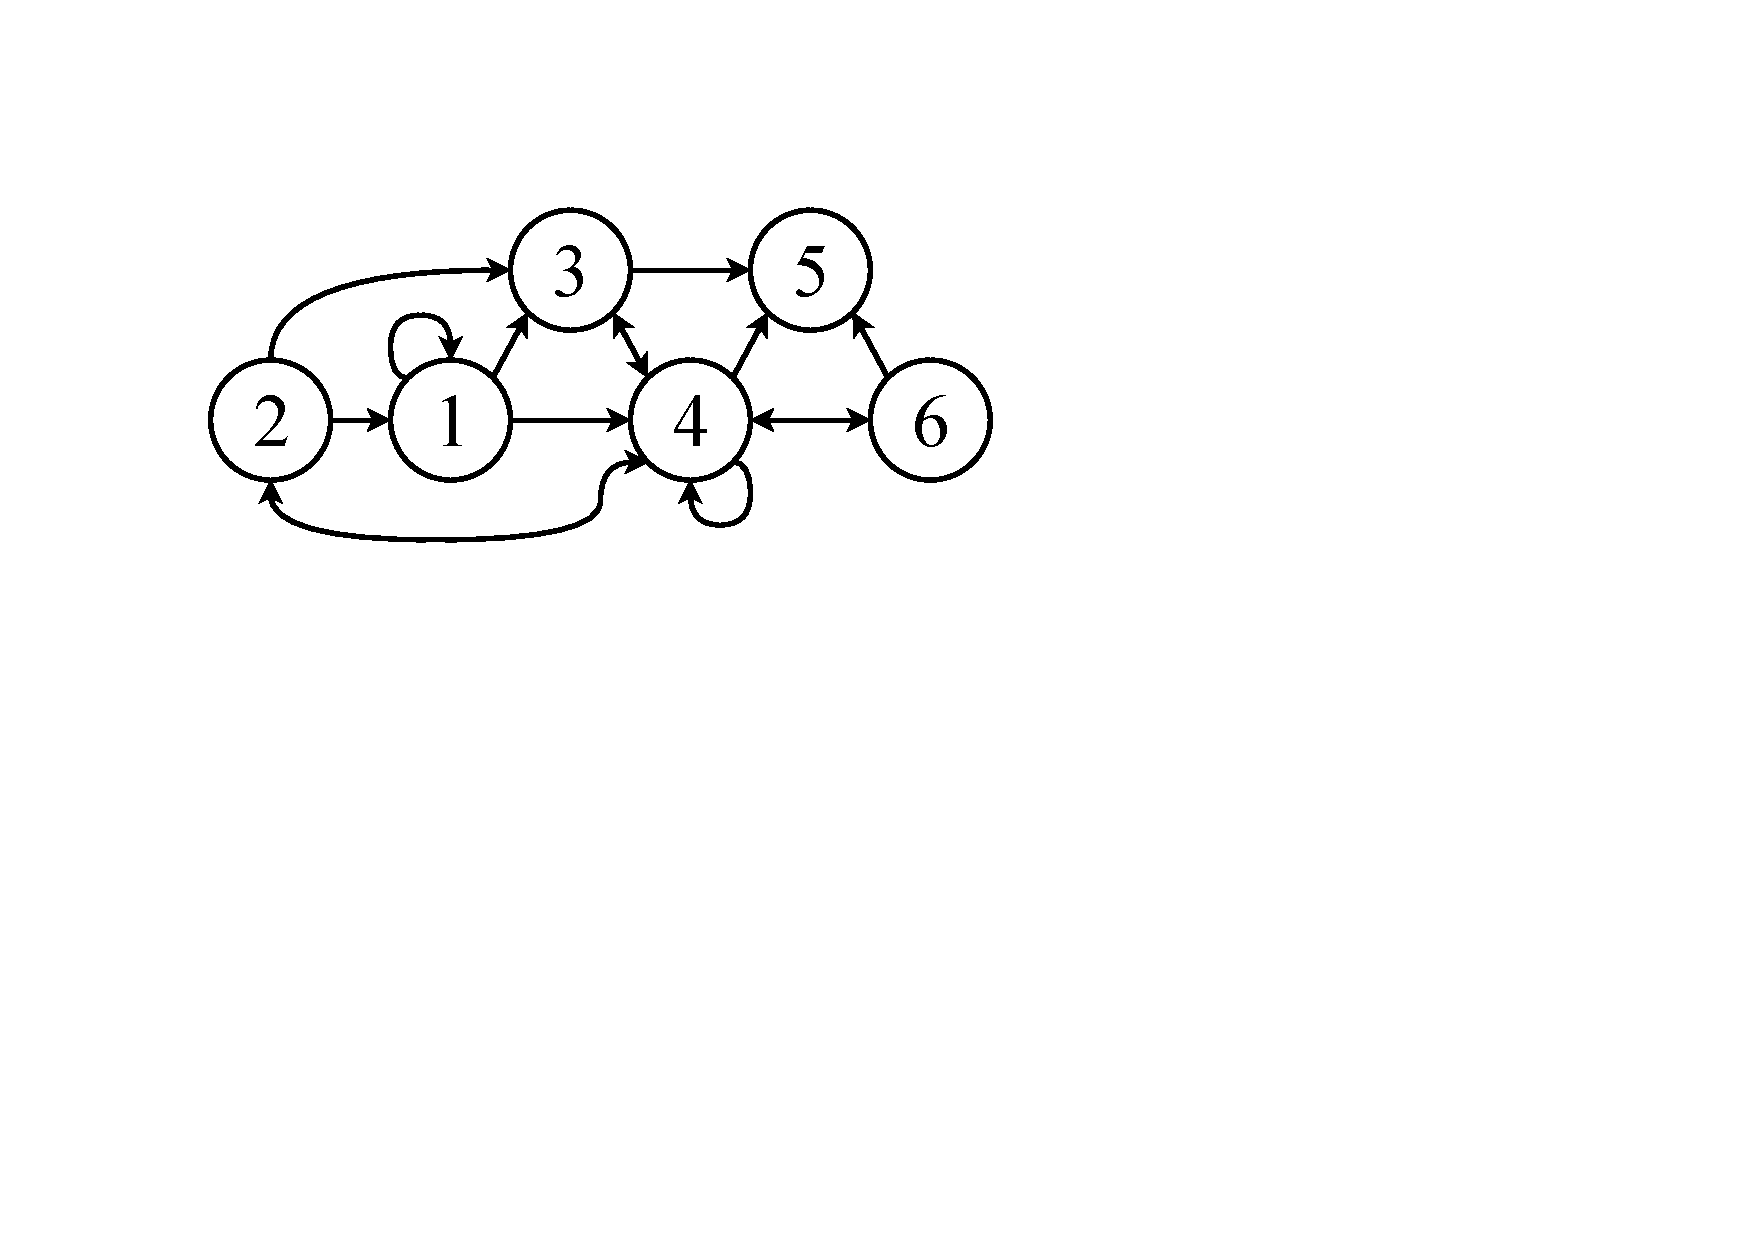
\includegraphics[scale=.3, clip,  trim=90 330 350 90]{img/arte/graphs-repair.pdf}
    		
    			(a)
    		\end{minipage}
    		\begin{minipage}{.35\textwidth}
    			\centering
    			\vspace{5mm}
		    	\begin{tabular}{|l|l|}
		    		\hline
		    		B1 & 111101 \\
		    		\hline
		    		B2 & 1111001\\
		    		\hline
		    	\end{tabular}
		    	\vspace{5mm}
		    	
    			(c)
    		\end{minipage}
    	\end{minipage}
    	\vspace{5mm}
    	
    	\begin{minipage}{1\textwidth}
    		\centering

		\begin{tabular}{l||l|l|l|l|l|l|l|l|l|l|l|l|l|l|l|l|l|l|l|l|l|}
			\toprule
			$T(G)$ & -1 & 1 & 3 & 4 & -2 & 1 & 3 & 4 & -3 & 4 & 5 & -4 & 3 & 4 & 5 & 6 & -5 & -6 & 4 & 5 \\
			\midrule
			$7 \rightarrow 4 \; 5$ & -1 & 1 & 3 & 4 & -2 & 1 & 3 & 4 & -3 & 7 & -4 & 3 & 7 & 6 & -5 & -6 & 7 \\
			\cline{1-18}
			$8 \rightarrow 1 \; 3$ & -1 & 8 & 4 & -2 & 8 & 4 & -3 & 7 & -4 & 3 & 7 & 6 & -5 & -6 & 7 \\
			\cline{1-16}
			$9 \rightarrow 8 \; 4$ & -1 & 9 & -2 & 9 & -3 & 7 & -4 & 3 & 7 & 6 & -5 & -6 & 7 \\
			\cline{1-14}
			Borrar $<0$ & 9 & 9 & 7 & 3 & 7 & 6 & 7 \\
			\cline{1-8}
		\end{tabular}				
		\vspace{5mm}
		
		(b)
    	\end{minipage}

    \caption{Ejemplo para Re-Pair aplicado a grafos por Claude y Navarro. (a) Grafo de ejemplo. (b) Listado concatenado $T(G)$ y resultado final luego de tres reemplazos y eliminar nodos de referencia. (c) Bitmaps indicadores de nodos de referencia removidos.}
    \label{fig:repairCN}
\end{figure}


Una propuesta de compresión más reciente, de Maneth y Peternek \cite{maneth2016compressing}, también generaliza Re-Pair para comprimir grafos, específicamente hipergrafos dirigidos.


\subsection{Virtual Node Mining, \textit{Buehrer y Chellapilla}}
Buehrer y Chellapilla \cite{BuehrerChellapilla} aprovechan que muchos grupos de nodos en el grafo de la Web consisten en conjuntos de sitios que comparten los mismas vecinos directos, lo que genera un grafo bipartito completo. Su propuesta reduce la cantidad de aristas, definiendo nodos virtuales que son agregados artificialmente al grafo entre los dos conjuntos del biclique. Esto reduce la cantidad total de aristas, ya que cada biclique une un set de $U$ nodos con uno de $W$ nodos, genera en total $|U \times W|$ aristas, y usando un nodo virtual disminuye a $|U + W|$, un gran ahorro cuando los bicliques son grandes. En la Figura~\ref{fig:virtualNode} se ejemplifica este reemplazo, cambiando de las iniciales 30 aristas del biclique en (a), 19 por un nodo virtual VN en (b), quedando solo 11 aristas restantes.

\begin{figure}%[b]
    	\centering
    	\begin{minipage}{0.45\textwidth}
    		\centering
    		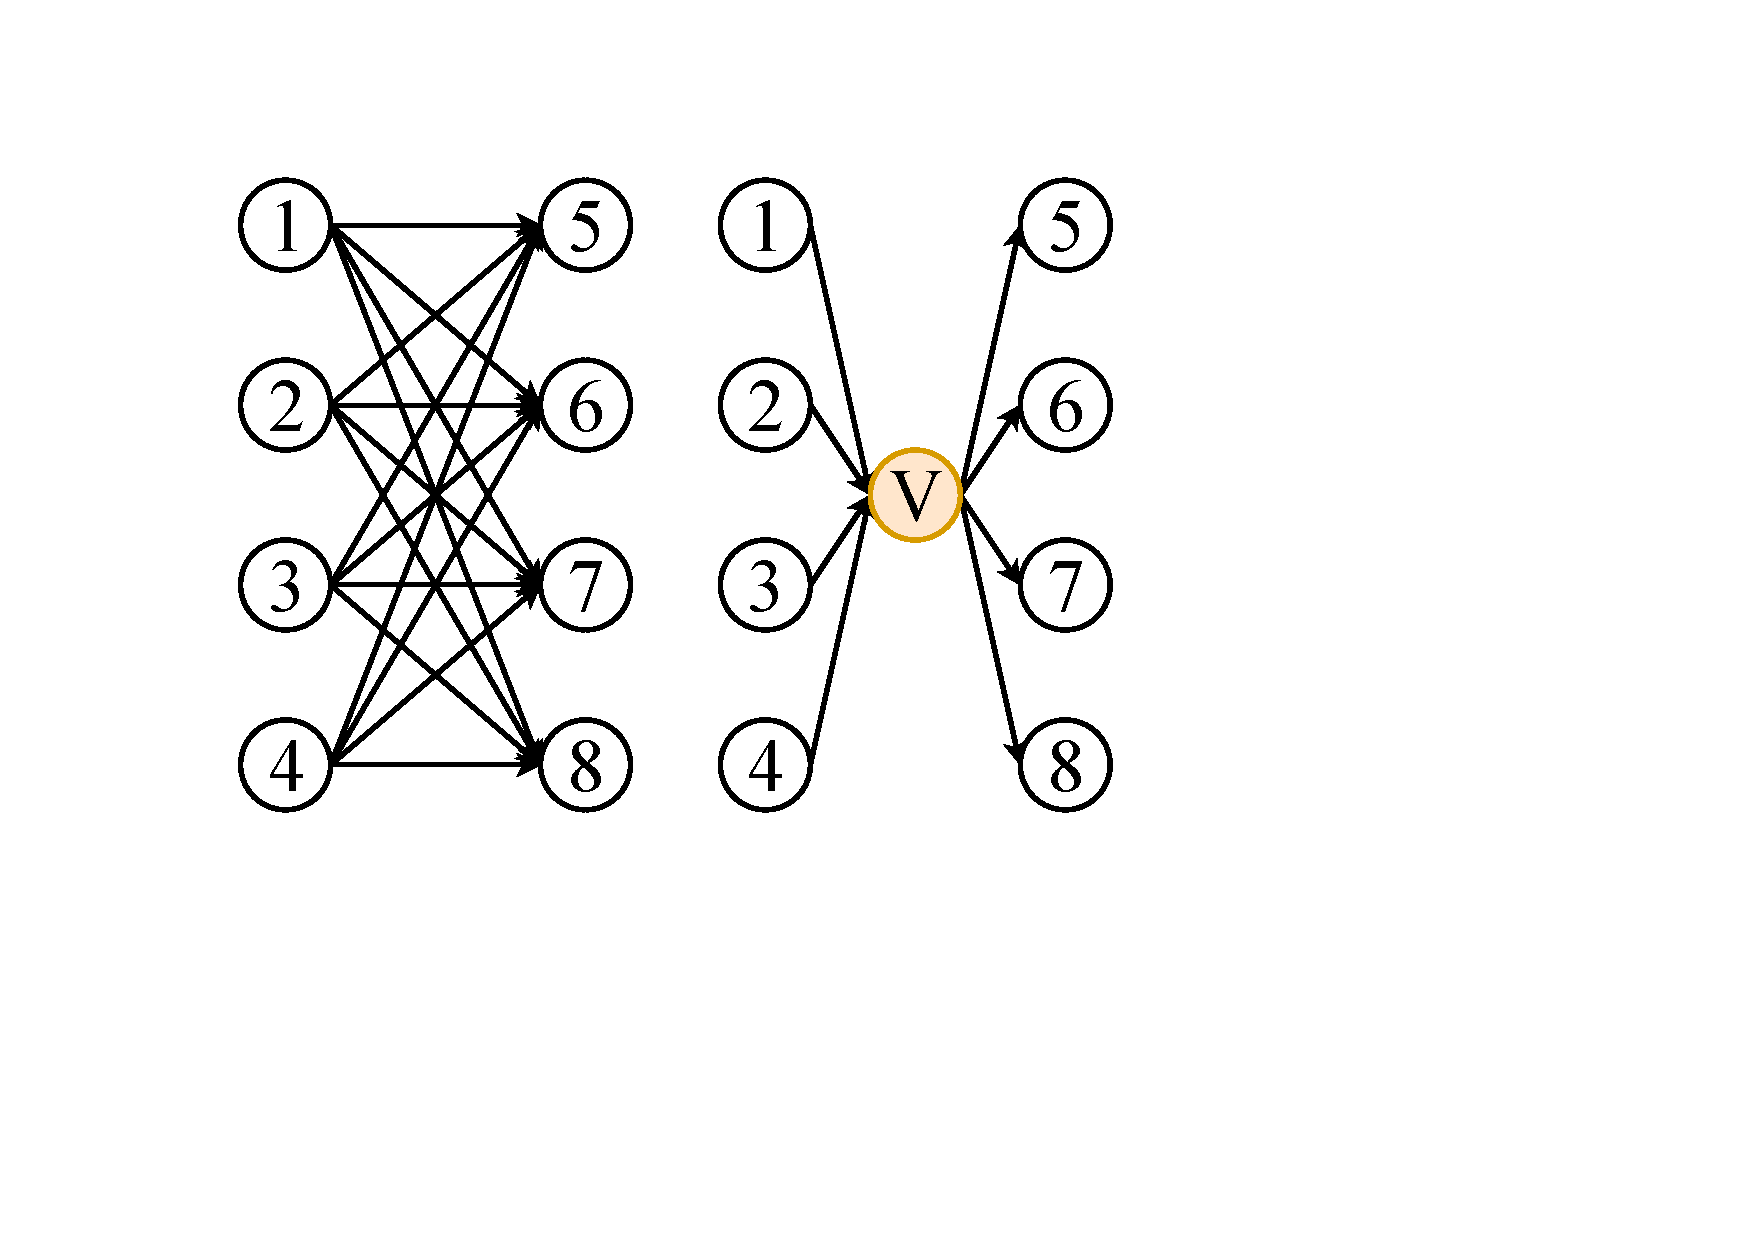
\includegraphics[scale=.3, clip,  trim=100 200 520 70]{img/arte/graphs-virtualNode.pdf}
    		
    		(a)
    	\end{minipage}
    	\begin{minipage}{0.45\textwidth}
    		\centering
    		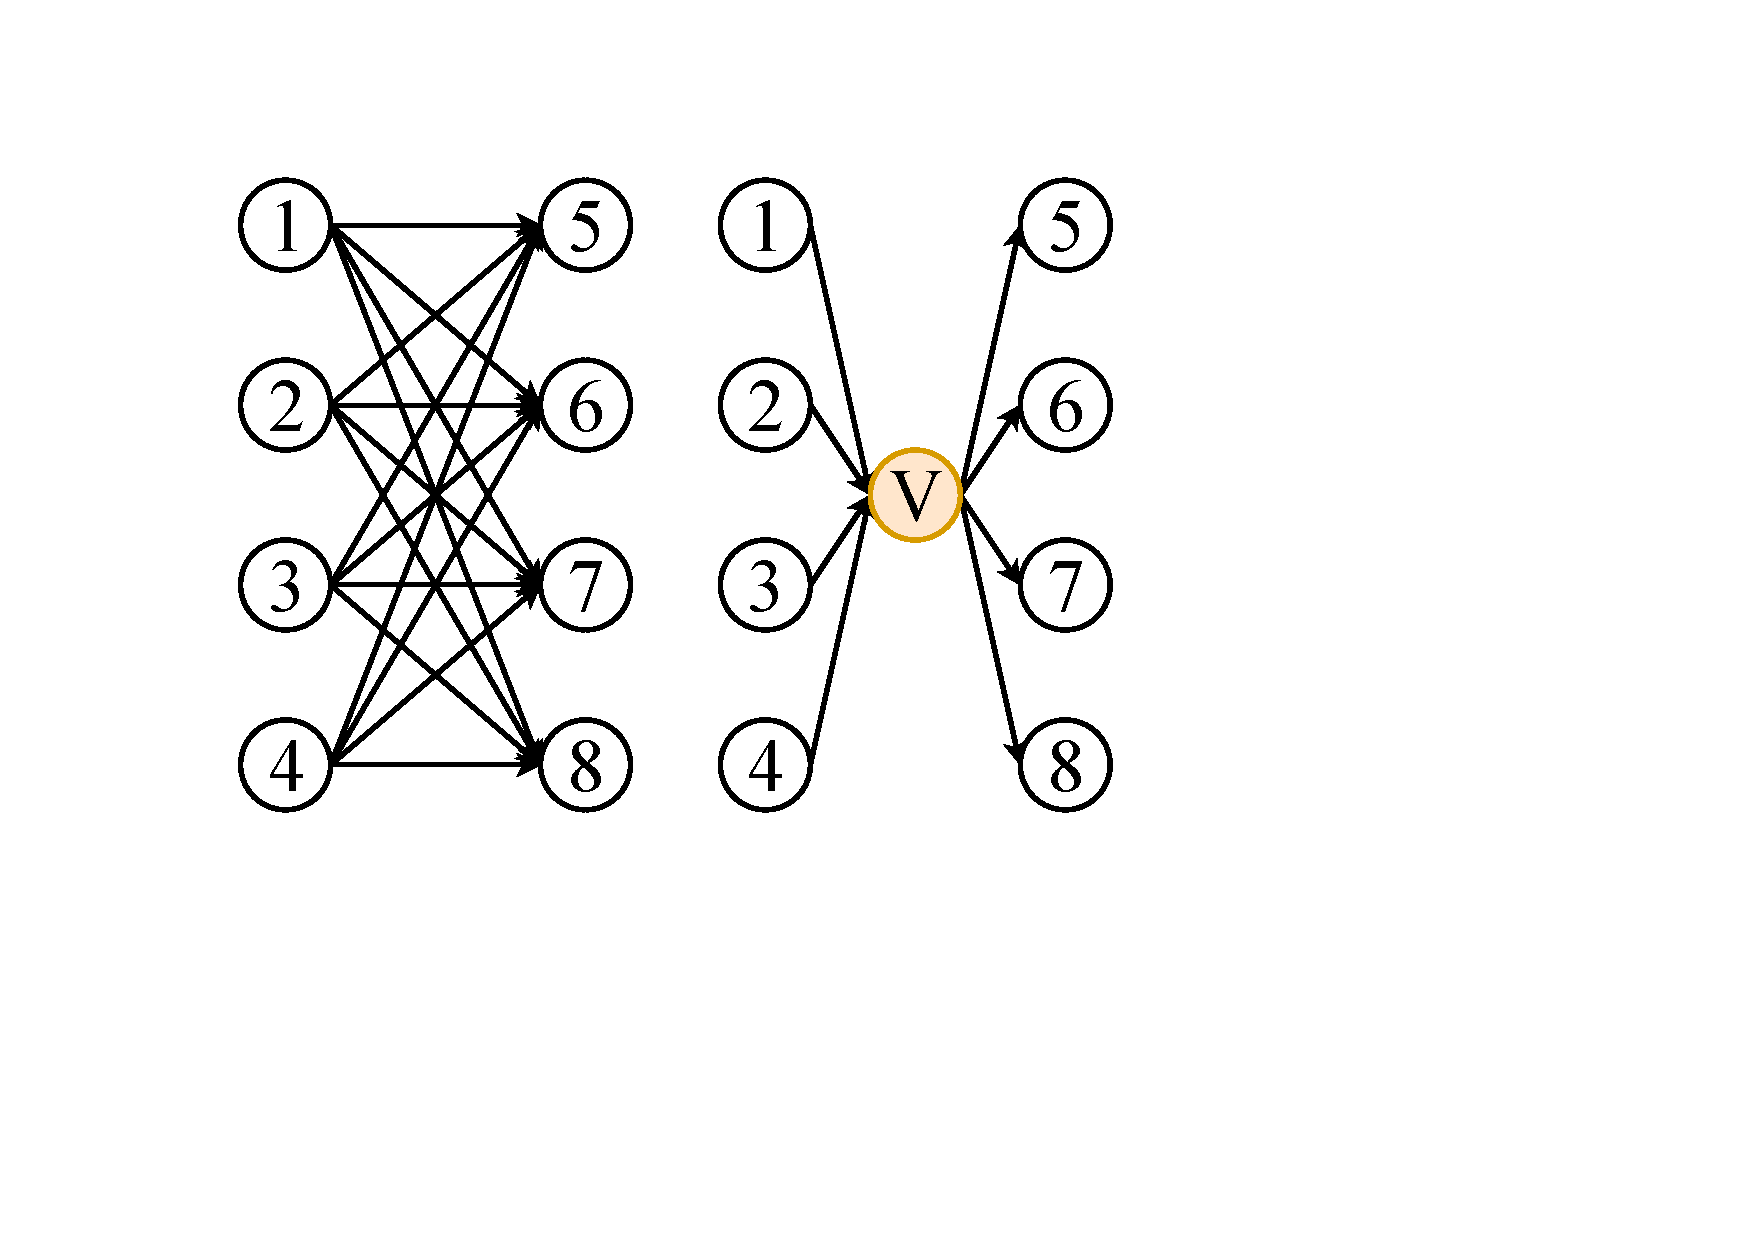
\includegraphics[scale=.3, clip, trim=330 200 290 70]{img/arte/graphs-virtualNode.pdf}
    		
    		(b)
    	\end{minipage}

    \caption{Ejemplo de reemplazo por nodo virtual. (a) Biclique. (b) Biclique con reemplazo de aristas por nodo virtual $V$.}
    \label{fig:virtualNode}
\end{figure}


Este proceso se repite iterativamente hasta que ya no se reducen significativamente más aristas. Luego aplican codificación delta (ver sección~\ref{sec:Ucoding}) sobre el grafo reducido. La propuesta logra una buena compresión, pero no reportan los tiempos de acceso. Además, su resultado no se ve afectado por el orden de numeración de los nodos, y permite actualizaciones.

Anh y Moffat \cite{anh2010local} también aprovechan esta localidad y similaridad en los listados de adyacencia, dividiendo en grupos de $h$ listas consecutivas. Luego reducen las listas aplicando reglas gramáticas como Re-Pair \cite{larsson2000off} de manera recursiva, y finalmente aplican codificaciones como el código $\zeta$ \cite{boldi2005codes}.


\subsection{k2-tree, \textit{Brisaboa, Ladra y Navarro}}
Una propuesta que aprovecha lo dispersa y agrupada que es la matriz de adyacencia del grafo de la Web es la propuesta por Brisaboa, Ladra y Navarro \cite{brisaboa2009k} donde proponen una estructura llamada k2-tree para ahorrar espacio y poder responder consultas tanto de vecinos directos como reversos. Esto último significa que este método, si bien fue pensado para grafos dirigidos, también se puede aplicar para no dirigidos. En un trabajo posterior, lograron mejorar sus resultados aplicando el ordenamiento por BFS antes de crear su estructura \cite{brisaboa2014compact}.

Este modelo propone representar la matriz de adyacencia con un árbol $k_{2}$-nario de altura $h=\lceil(\log_k n)\rceil$, donde $n$ es el número de vértices en el grafo. Luego subdivide la matriz de adyacencia en $k^2$ submatrices de tamaño $n^{2}/k^{2}$, si una de ellas contiene solo ceros se representa solo con un bit en $0$, de lo contrario se marcan con un $1$ y se vuelven a subdividir de manera recursiva. Esta estructura soporta las consultas de vecinos directos y reversos de manera simétrica, ya que significa revisar las filas o columnas de la matriz. En la Figura~\ref{fig:k2tree} se presenta (a) un ejemplo de una matriz de adyacencia y sus subdivisiones para k2tree, y (b) un diagrama de la estructura final.

\begin{figure}%[b]
    	\centering
    	\begin{minipage}{0.45\textwidth}
    		\centering
    		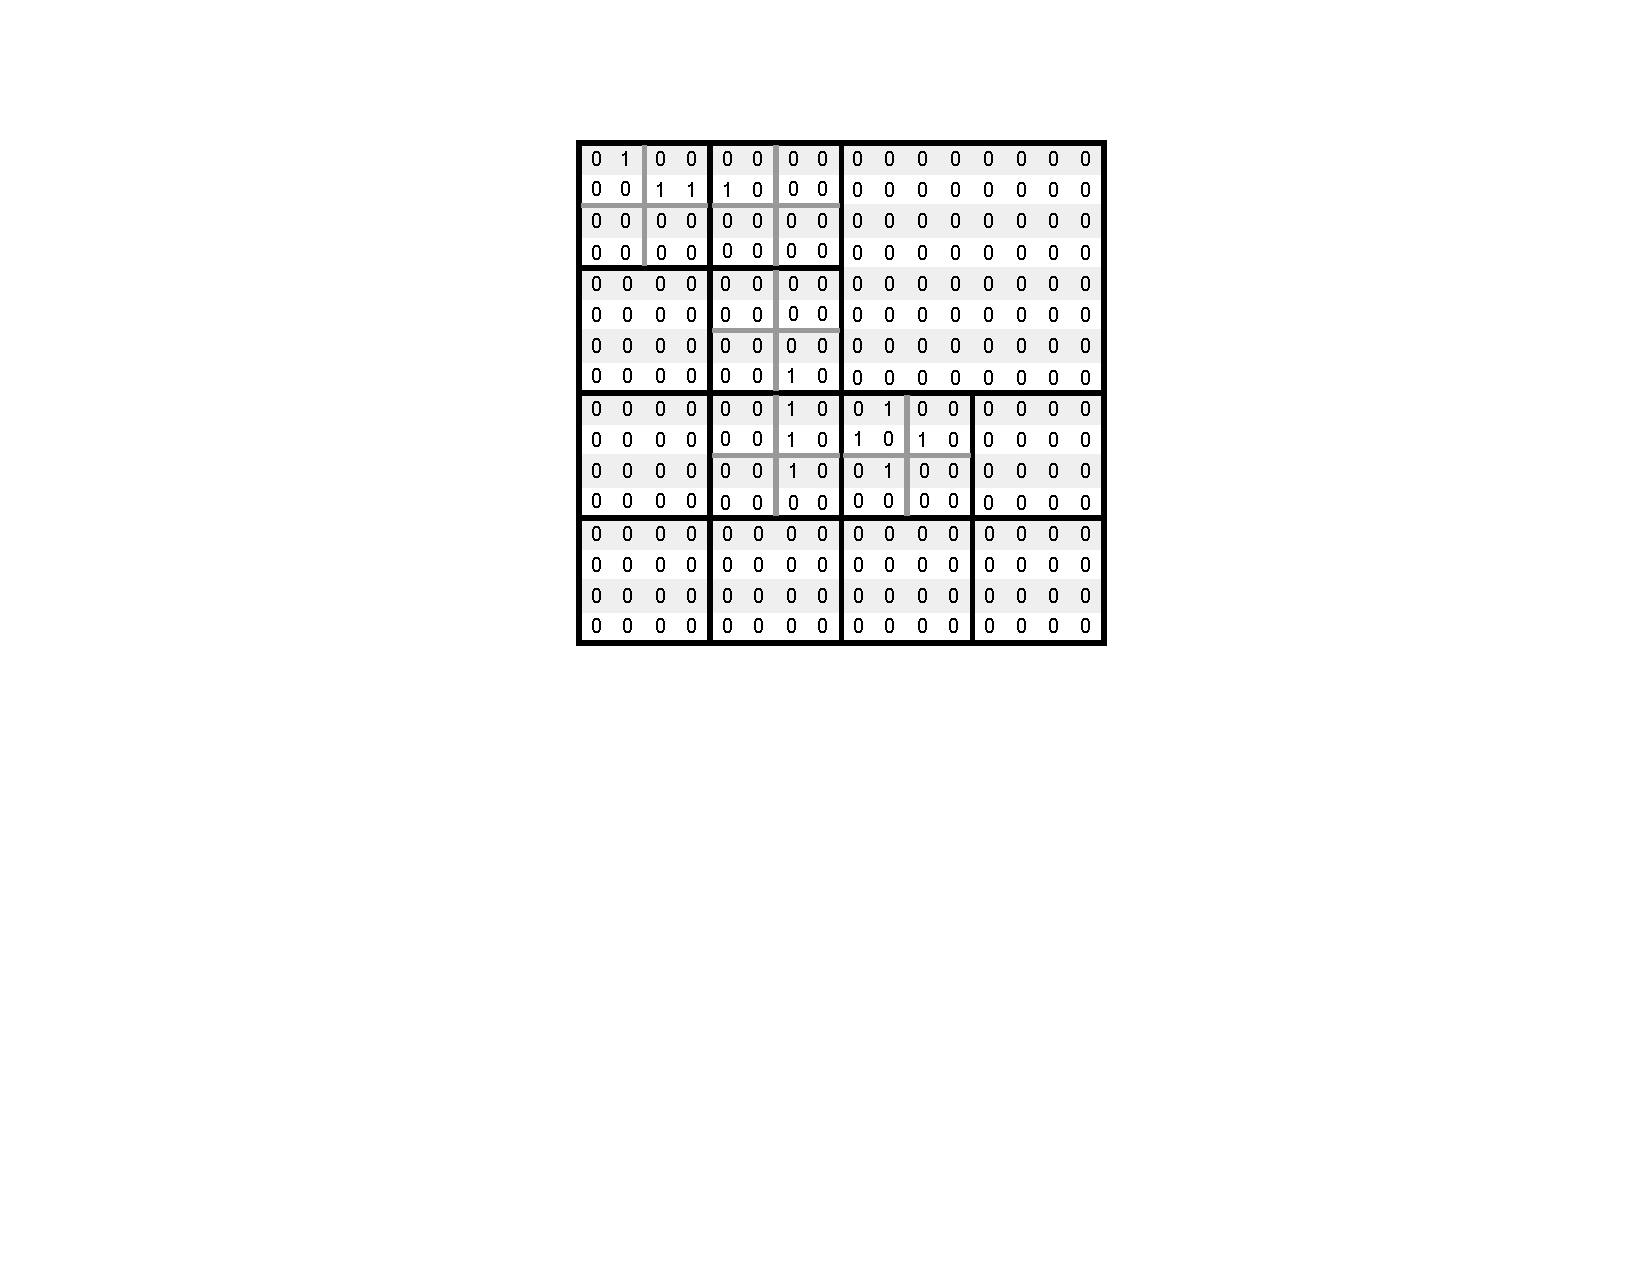
\includegraphics[scale=.6, clip,  trim=270 280 250 0]{img/arte/k2-tree-matrix.pdf}
    		
    		(a)
    	\end{minipage}
    	\begin{minipage}{0.45\textwidth}
    		\centering
    		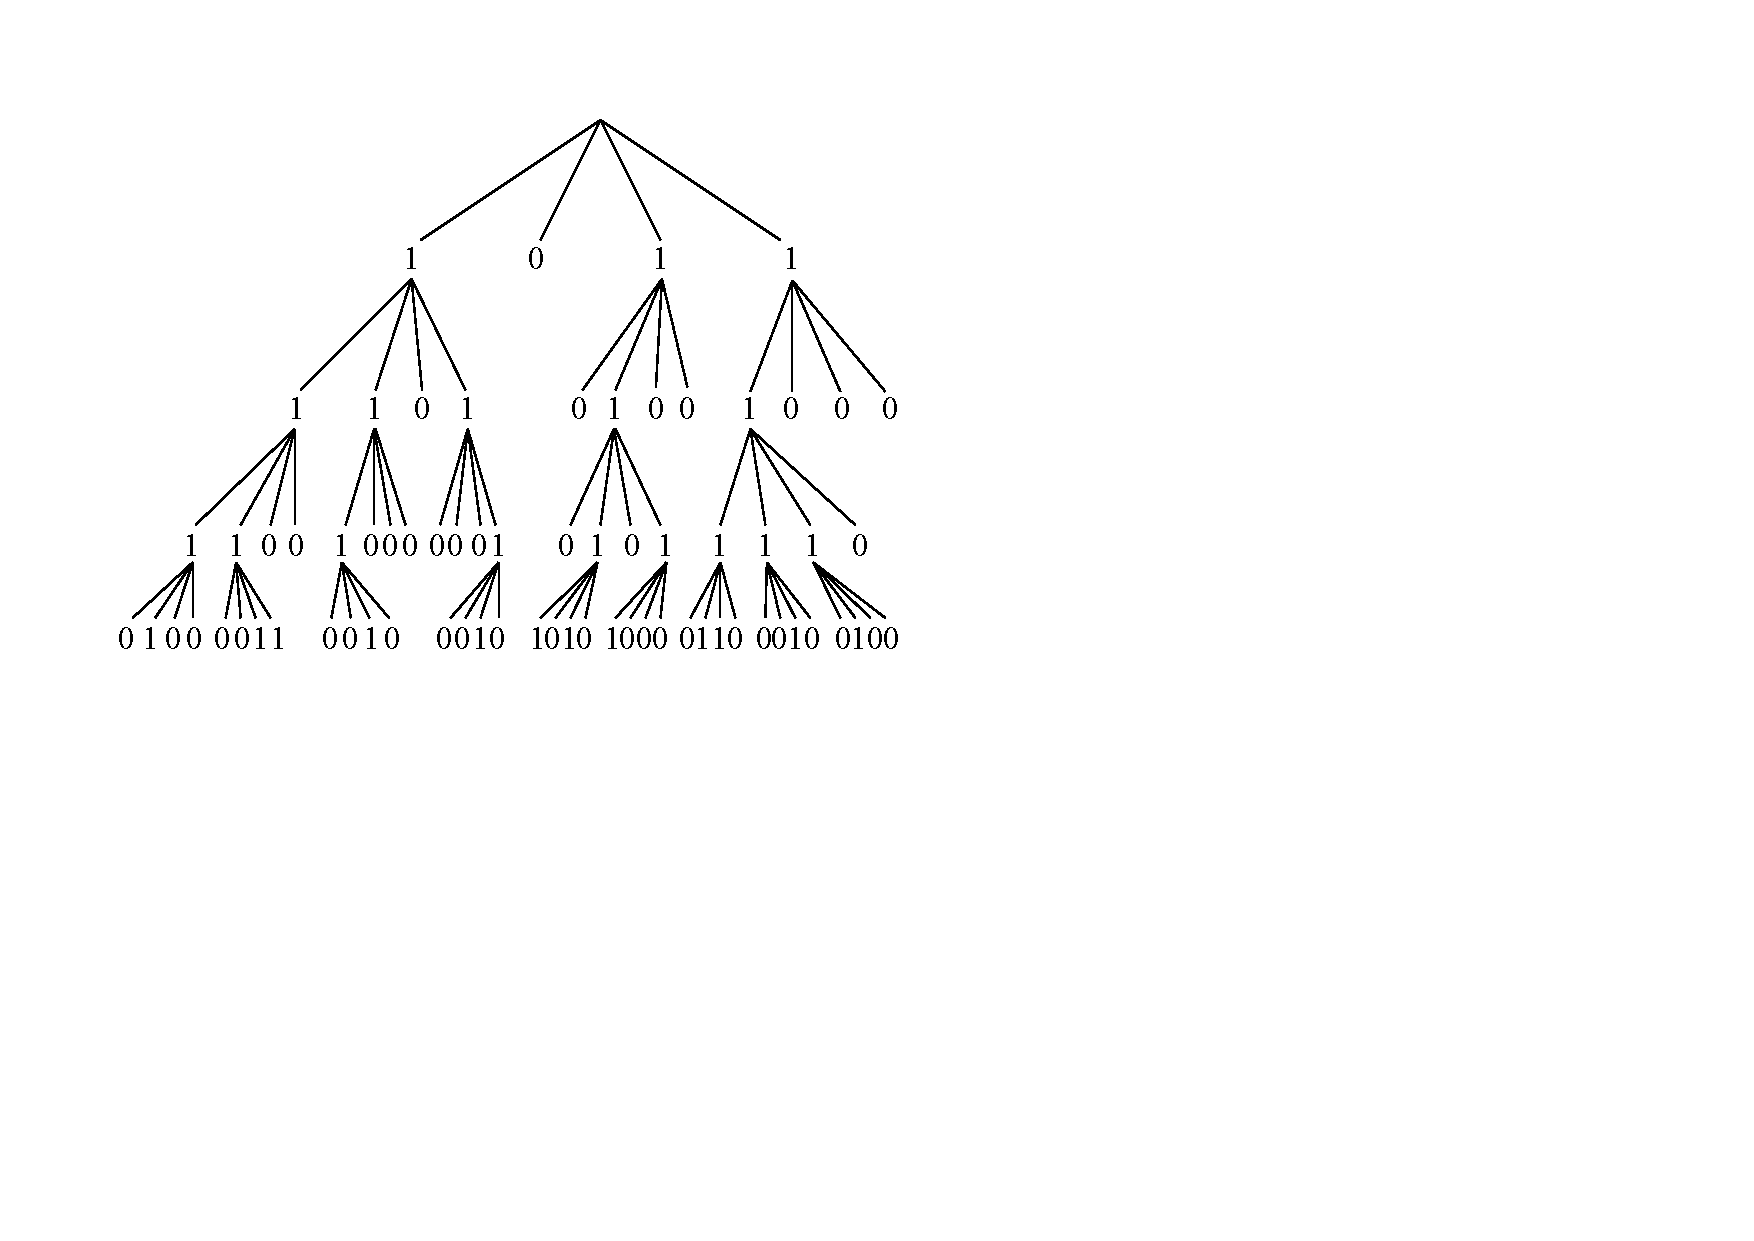
\includegraphics[scale=.5, clip, trim=50 280 410 0]{img/arte/graphs-k2tree.pdf}
    		
    		(b)
    	\end{minipage}

    \caption{Ejemplo de k2-tree. (a) Matriz de adyacencia. (b) Diagrama de estructura.}
    \label{fig:k2tree}
\end{figure}


Finalmente, la compresión se realiza representando el árbol usando dos arreglos de bits, un bitmap $T$ para representar la estructura del árbol, y un bitmap $L$ para representar las hojas, que representan las celdas de la matriz. Además usan un bitmap adicional para acelerar la resolución de consultas. 

En 2011, Hernández y Navarro \cite{hernandez2011compression} propusieron combinar varios métodos: Primero reducir la cantidad de aristas con nodos virtuales \cite{BuehrerChellapilla},  y luego comprimir usando las propuestas de k2-tree \cite{brisaboa2009k} y el trabajo anterior basado en Re-Pair \cite{claude2010fast}, logrando resultados de compresión bastante competitivos, pero sacrificando tiempos de acceso. En trabajos posteriores, Hernandez y Navarro \cite{hernandez2012compressed, hernandez2014compressed} proponen una estructura bastante similar, pero los bicliques son representados usando estructuras sucintas como wavelet trees y bitmaps comprimidos (ver Sección \ref{sec:compactEstruct}). Esta representación comprimida proporciona resolución de consulta de vecinos directos y reversos. Francisco et. al. \cite{francisco2018exploiting} destacan que esta propuesta también presenta un formato adecuado para potenciar los cálculos de cómputo de matrices por vectores.



%Una propuesta muy reciente, por Li et. al.\cite{li2019optimal} mejora considerablemente k2-tree proponiendo una manera distinta de subdividir la matriz de adyacencia.

\subsection{List Merging, \textit{Grabowski y Bieniecki}}
Grabowski y Bieniecki proponen agrupar los listados de adyacencia en bloques de $h$ listas cada uno, de manera similar a lo propuesto por Anh y Moffat \cite{anh2010local}. Cada bloque luego es descompuesto en dos arreglos: el primero es \textit{long list}, un arreglo de todos los índices de los vértices presentes en el bloque de listados de adyacencia, sin repetir ninguno. El segundo es \textit{flags}, un arreglo de bits que permite la reconstrucción de las listas agrupadas. 

El arreglo de enteros \textit{long list} es reducido usando las diferencias, terminada en cero y codificada en bytes. El arreglo de bits \textit{flags} indica la pertenencia de los índices en \textit{long list} a sus listas de adyacencias asociadas. El número de bits por cada índice es $h$, definido como un múltiplo de 8. su largo queda definido por el largo de \textit{long list}. Este arreglo puede no comprimirse (en cual caso lo llaman \textit{LM-bitmap}), o codificarse usando las diferencias entre los 1 sucesivos, escritas en bytes individuales (\textit{LM-diff}).

Ambas secuencias, \textit{long list} y ya sea \textit{LM-bitmap} o \textit{LM-diff}, luego son concatenadas y comprimidas usando el algoritmo Deflate. Este algoritmo consiste en una serie de bloques, todos precedidos por una cabecera de 3 bits, que indican lo siguiente:

\begin{itemize}
	\item Primer bit:
	\begin{itemize}
		\item 0: No es el último bloque de la secuencia.
		\item 1: Es el último bloque de la secuencia.
	\end{itemize}
	\item Segundo y tercer bit:
	\begin{itemize}
		\item 00: Bloque sin codificar.
		\item 01: Bloque codificado con Huffman, con un árbol de Huffman ya definido.
		\item 10: Bloque codificado con Huffman y su árbol asociado.
		\item 11: Reservado; No usar.
	\end{itemize}
\end{itemize}

Para más detalles sobre la codificación Huffman, ver la Sección~\ref{sec:huffman}.


\subsection{GLOUDS, \textit{Fischer y Peters}}
Fischer y Peters \cite{fischer2016glouds} proponen una nueva estructura de datos sucintos para comprimir grafos con forma de árbol, llamada \textit{GLOUDS (Graph Level Order Unary Degree Sequence)}. La idea del algoritmo es representar mediante otra estructura de datos sucintos para árboles de expansión, llamada \textit{LOUDS (Level Order Unary Degree Sequence)} \cite{jacobson1989space}, y agregarle información adicional para los nodos extra.

\begin{figure}%[b]
    	\centering
    	\begin{minipage}{0.25\textwidth}
    		\centering
    		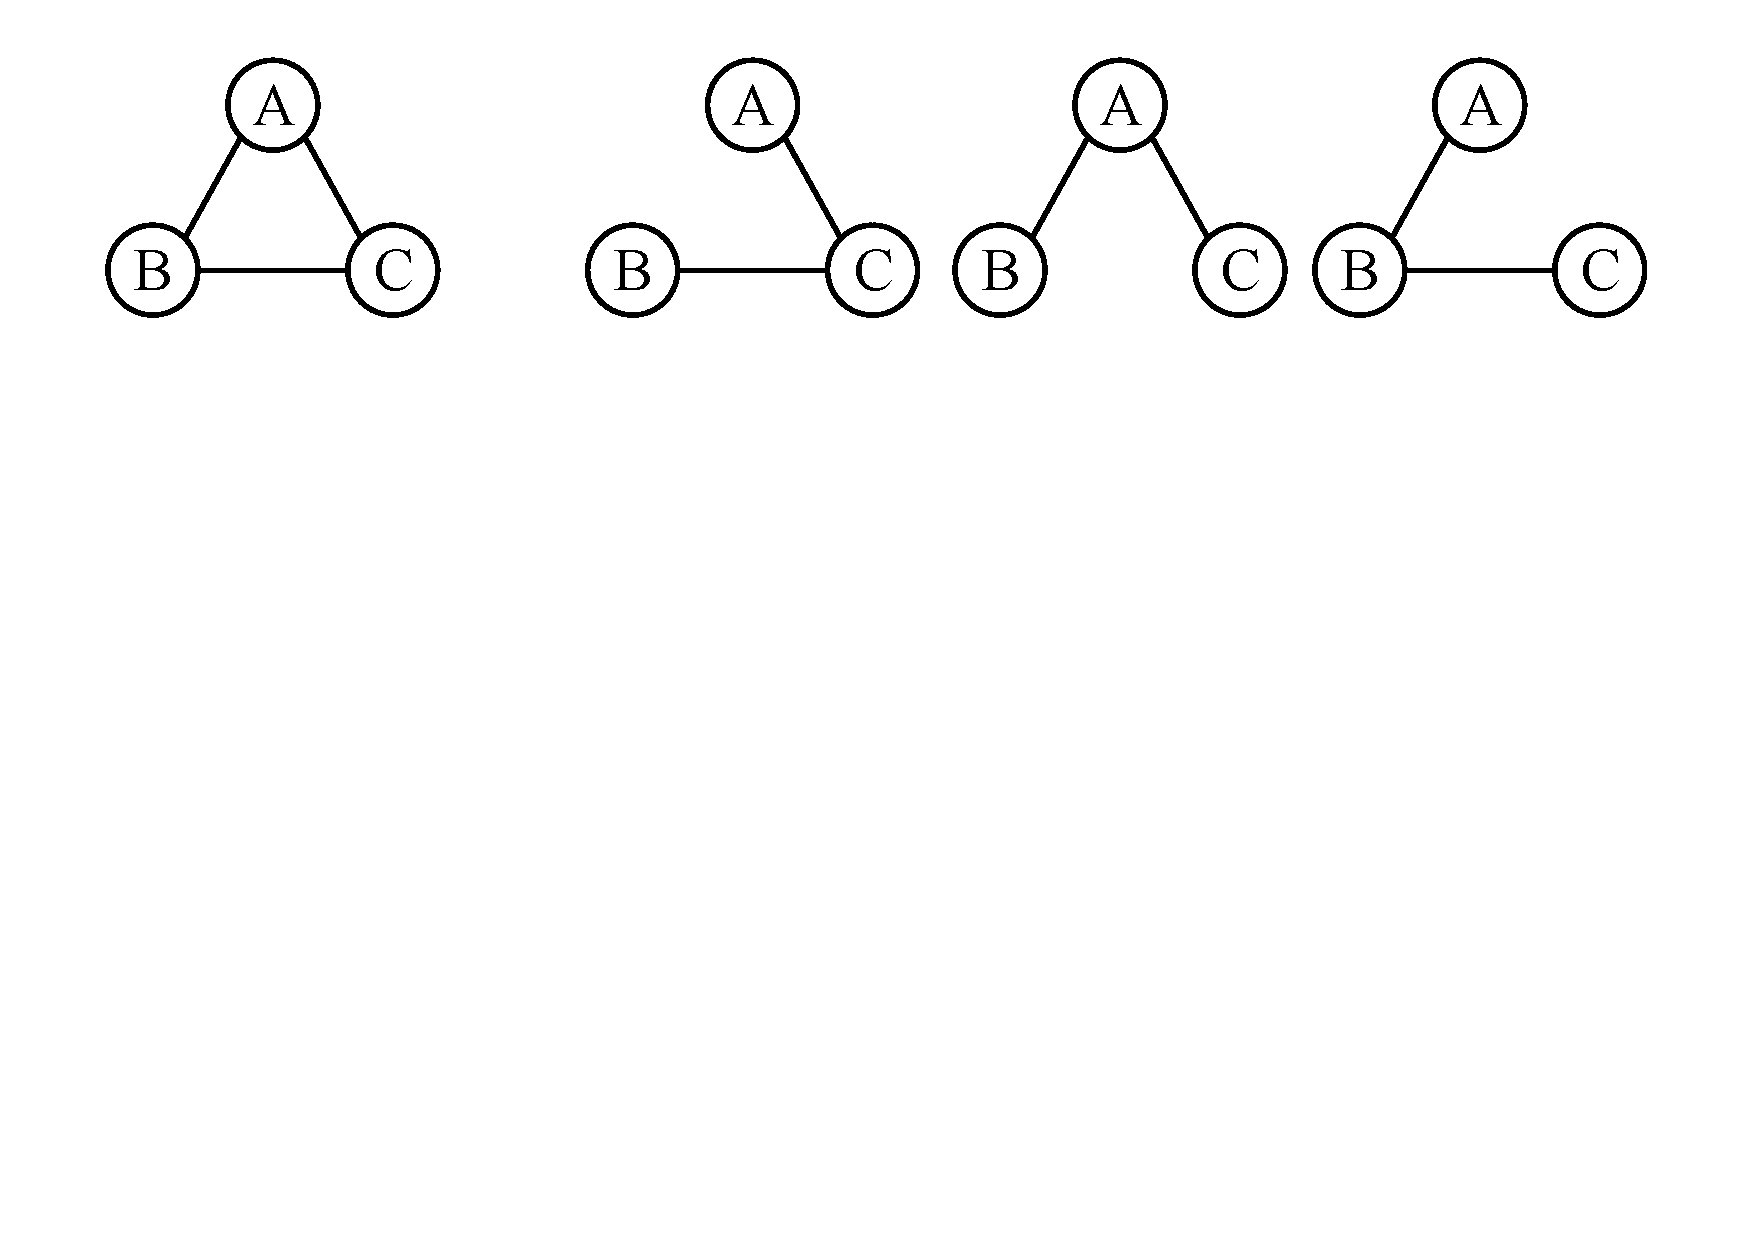
\includegraphics[scale=.4, clip,  trim=50 440 630 20]{img/arte/graphs-spanningTree.pdf}
    		
    		(a)
    	\end{minipage}
    	\begin{minipage}{0.65\textwidth}
    		\centering
    		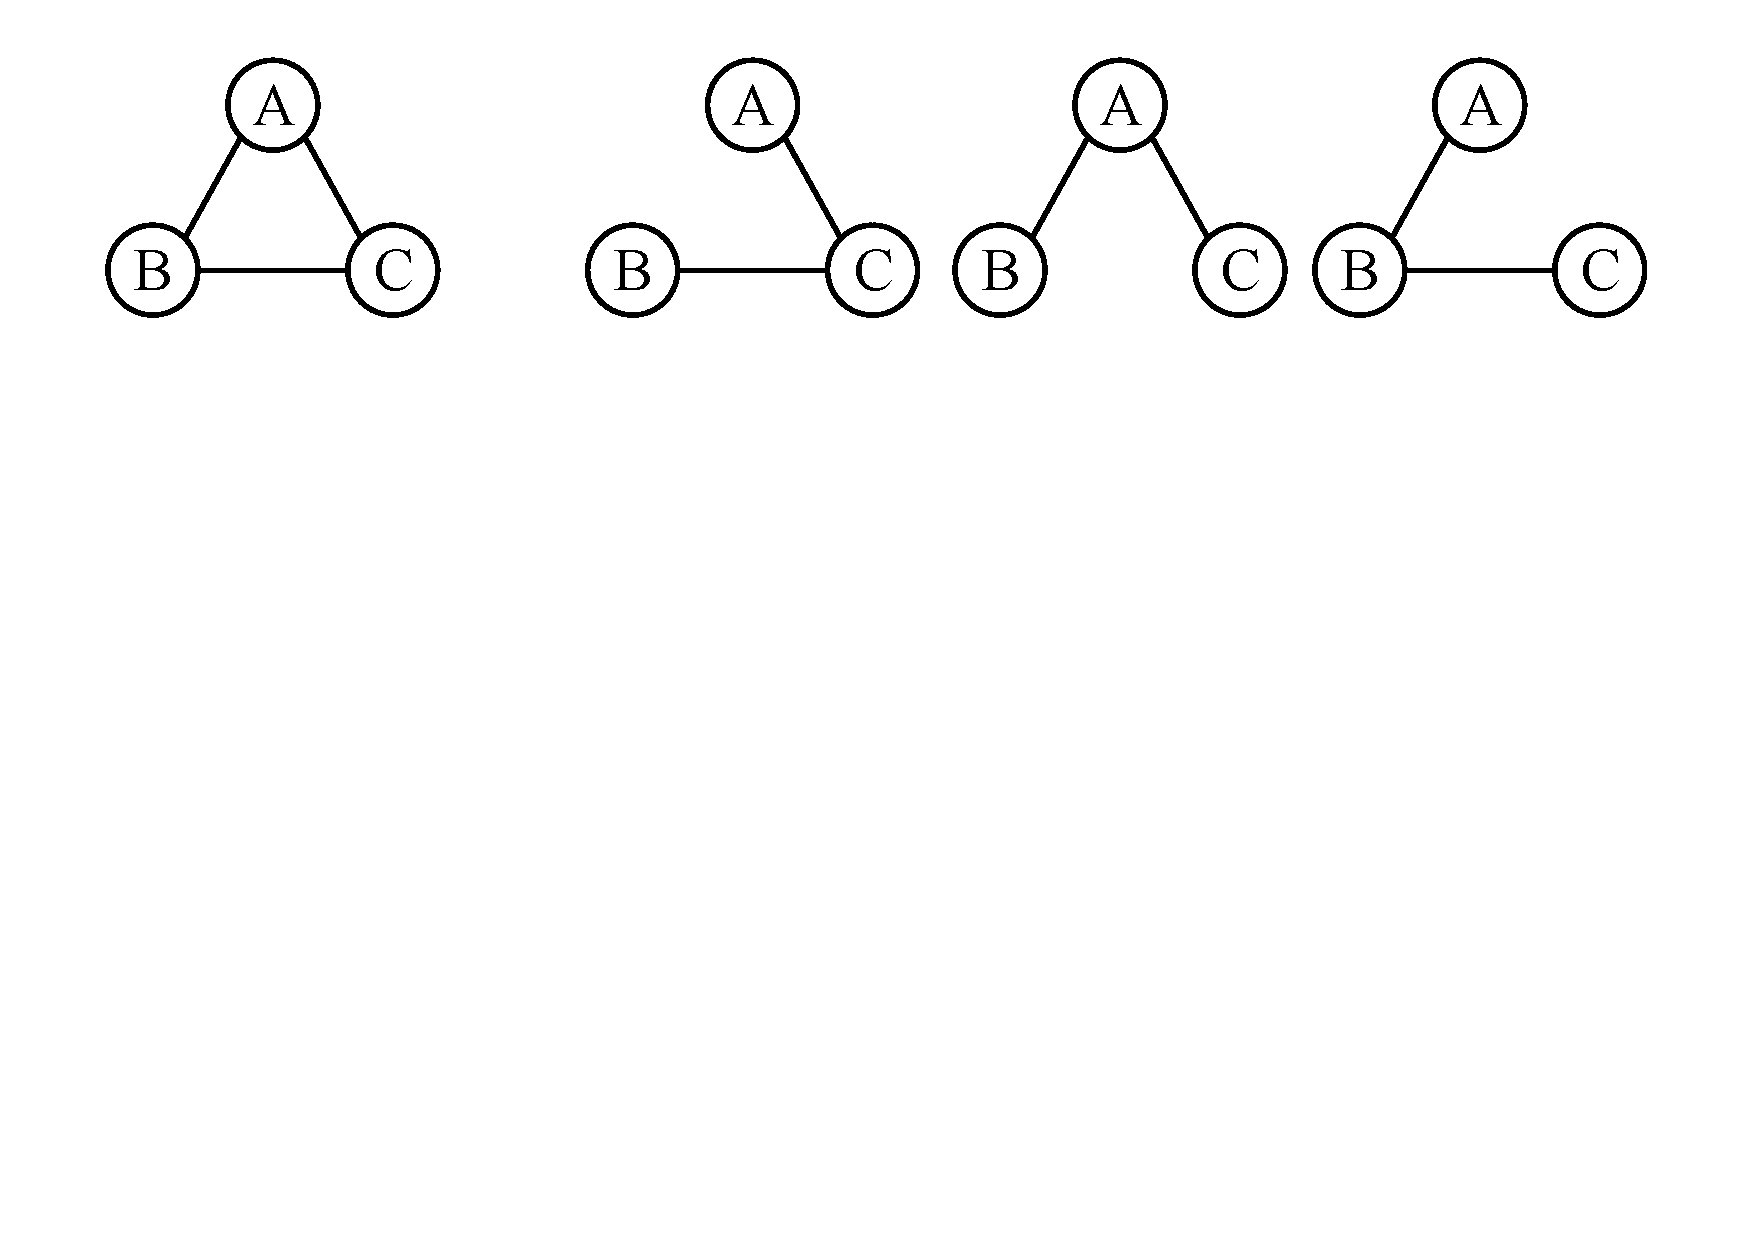
\includegraphics[scale=.4, clip, trim=280 440 50 20]{img/arte/graphs-spanningTree.pdf}
    		
    		(b)
    	\end{minipage}

    \caption{Ejemplos de árboles de expansión. (a) Grafo simple. (b)~Posibles árboles de expansión para el grafo.}
    \label{fig:spanningTree}
\end{figure}


\begin{figure}%[b]
    	\centering
    	\begin{minipage}{0.45\textwidth}
    		\centering
    		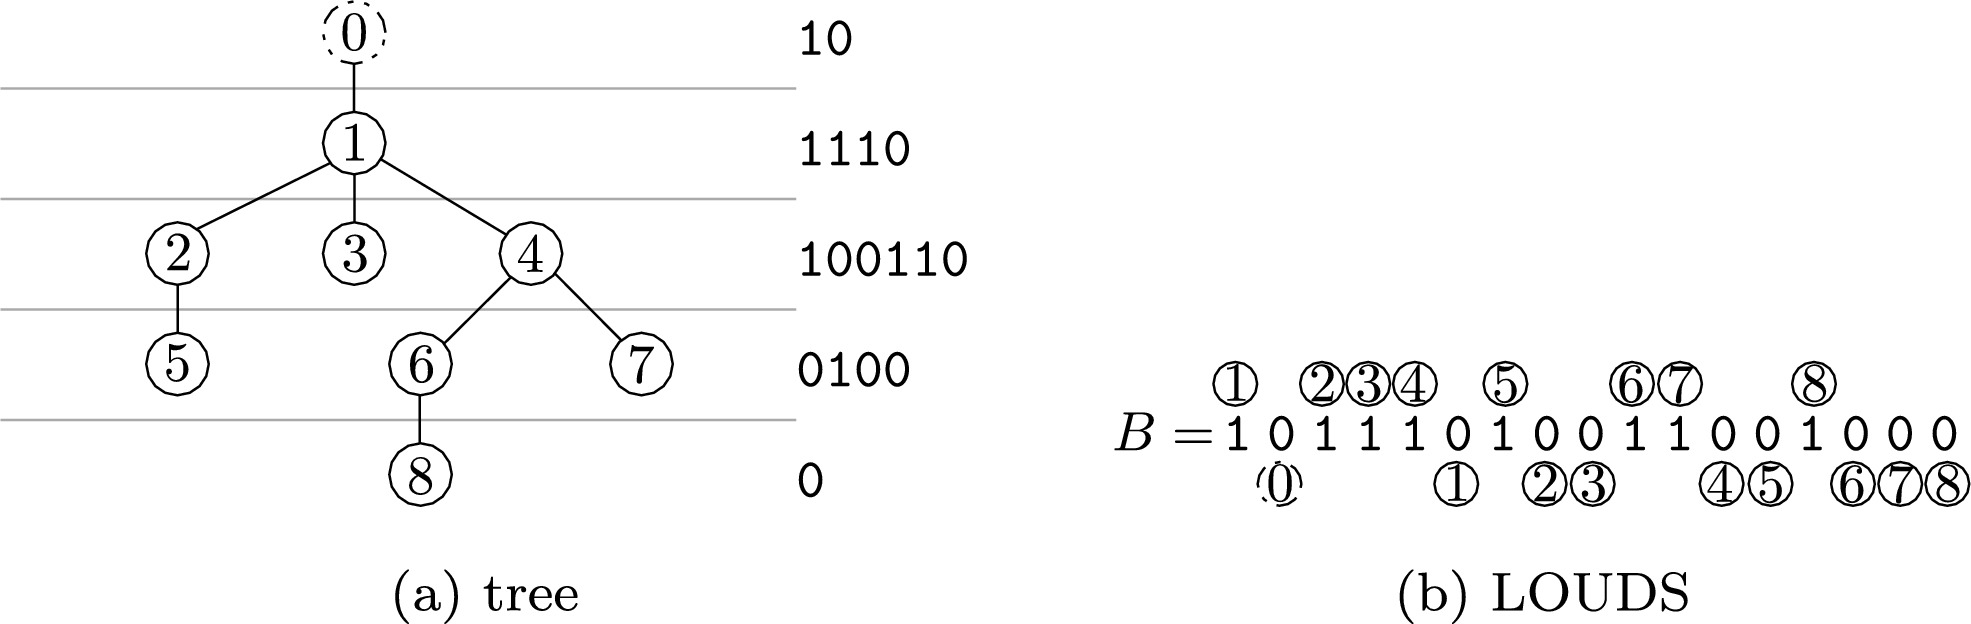
\includegraphics[scale=1.6, clip,  trim=10 16 140 0]{img/arte/LOUDS.jpg}
    		
    		(a)
    	\end{minipage}
    	\begin{minipage}{0.45\textwidth}
    		\centering
    		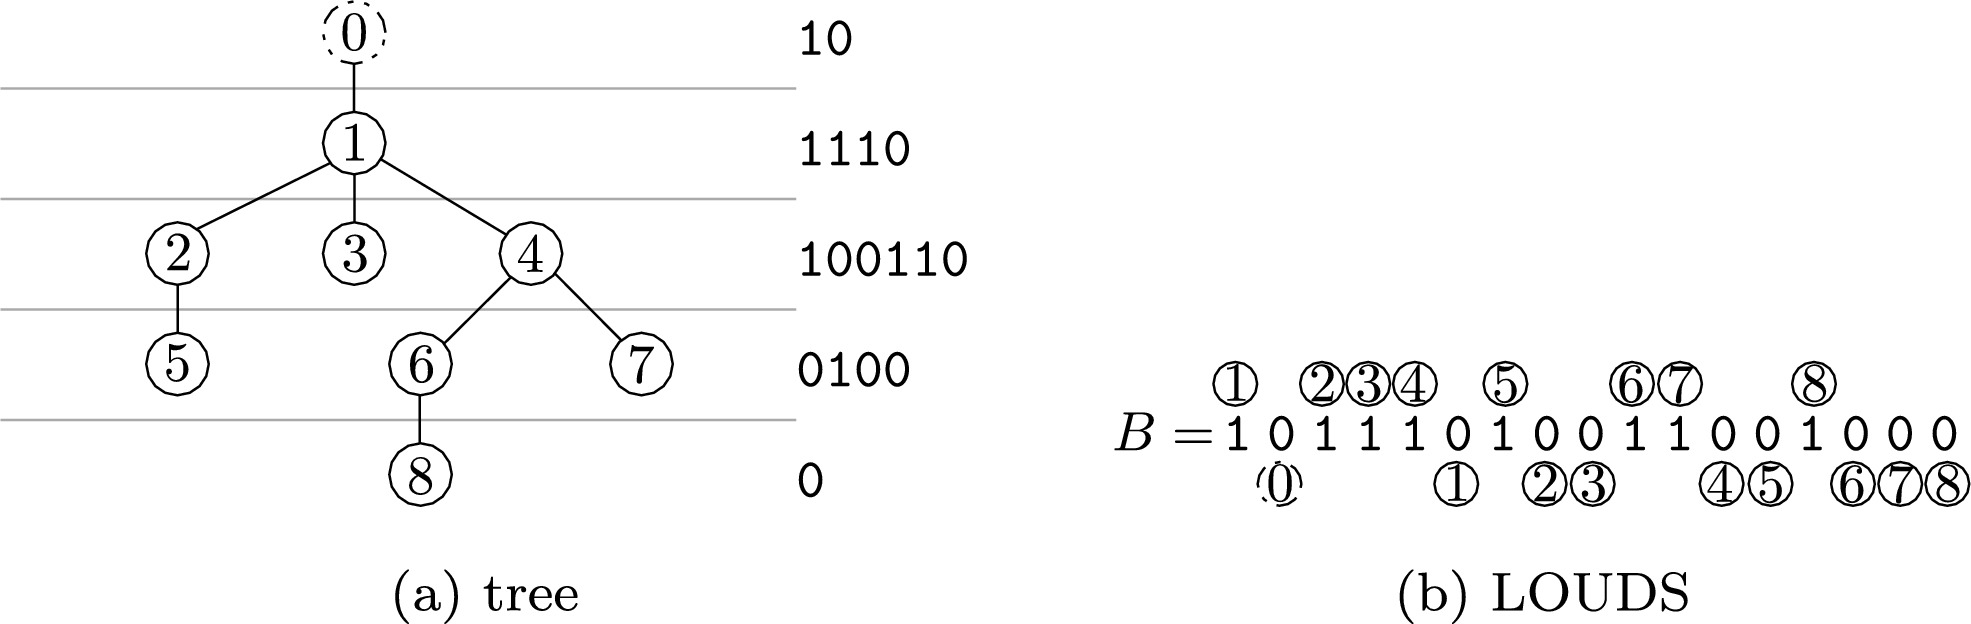
\includegraphics[scale=1.6, clip, trim=150 16 0 50]{img/arte/LOUDS.jpg}
    		
    		(b)
    	\end{minipage}

    \caption{Ejemplo de un árbol de expansión y su LOUDS. (a) Árbol de expansión y los bits generados por cada nivel de BFS. (b)~Bitmap $B$ de LOUDS.}
    \label{fig:LOUDS}
\end{figure}


Un árbol de expansión $T$ de un grafo $G$  con $n$ vértices y $m$ aristas, es un árbol que cubre todos los $n$ vértices de $G$ con la mínima cantidad de aristas posibles, sin generar ciclos. En la Figura~\ref{fig:spanningTree} se muestran algunos ejemplos de árboles de expansión para un grafo simple. Un grafo con forma de árbol no tiene una cantidad de aristas adicionales muy alta, con respecto a un árbol de expansión.

La estructura \textit{LOUDS} \cite{jacobson1989space} está diseñada para comprimir árboles de expansión. Primero, por conveniencia, agrandan el árbol con un nodo \textit{super-raíz} artificial conectado al nodo raíz original. Luego van construyendo un bitmap $B$, avanzando por el árbol mediante BFS. Por cada nodo con $k$ hijos, se agregan $1^{k}0$ bits a $B$ (con $k=3$ sería $1110$). Esto representa a cada nodo del árbol dos veces: una vez con un $1$ cuando aparece el nodo como hijo, y con un $0$ cuando aparece como padre. Para $n$ nodos, el bitmap $B$ tiene $2n + 1$ bits de largo. En la Figura~\ref{fig:LOUDS} se muestra un ejemplo de esta representación. Los nodos quedan identificados según el nivel de BFS donde aparecen.

Basado en esta idea, \textit{GLOUDS} \cite{fischer2016glouds} propone una nueva estructura para grafos con forma de árbol. Para esto define las siguientes características de un grafo $G$:

\begin{itemize}
	\item $c \leq n$, la cantidad de nodos raíz de $G$ (el tamaño mínimo del set de nodos desde donde se alcanzan todos los nodos restantes). 
	\item $k = m - n + 1$, la cantidad de aristas adicionales, con respecto al árbol de expansión $T$ de $G$.
	\item $h \leq k$, la cantidad de nodos adicionales.
\end{itemize}

Por simpleza, parten asumiendo que existe un nodo $r$ desde donde se pueden alcanzar todos los nodos restantes ($c = 1$). Desde $r$, realizan el recorrido por BFS de $G$, lo que llaman BFT, y $T_{G}^{BFT}$ el árbol resultante. Agrandan $T_{G}^{BFT}$ tal que por cada vértice $w$ ya visitado durante la BFT del nodo $v$ en una etapa anterior, realizan una copia llamada \textit{nodo sombra} y la agregan como hijo al nodo $v$ en $T_{G}^{BFT}$. Finalmente agregan el nodo \textit{super-raíz}, y llaman al árbol final $T_{G}$, que tiene exactamente $m + 2$ nodos. En la Figura~\ref{fig:GLOUDS} se ilustra un ejemplo de GLOUDS, en (a) el grafo $G$, y en (b) el árbol $T_{G}$ final.

\input{figs/arte-glouds}

Luego proponen una representación de $T_{G}$ similar a la de LOUDS, pero que permita diferenciar los nodos sombra de los demás. Para esto, cambian el bitmap por una secuencia de trits, con posibles valores del conjunto $\{0, 1, 2\}$. Luego, la secuencia $B$ se genera de la misma manera, pero cuando aparece un nodo sombra en el recorrido BFS se agrega un $2$. Estos nodos no se vuelven a representar con un $0$. Le llaman al vector de trits $B$ CLOUDS, y tiene un largo de $n + m + c$ trits. En la Figura~\ref{fig:LOUDS}~(c) se muestra el resultado para el ejemplo ya mencionado. Además, necesita un arreglo $H[0, k)$ que anota los nodos sombra que aparecen en B.



\section{Estructuras compactas} \label{sec:compactEstruct}
En esta sección se detallan las posibles estructuras compactas basadas en secuencias que se evaluarán para la compresión de la estructura planteada. Las operaciones básicas que permiten son \textbf{$Rank$}, \textbf{$Select$} y \textbf{$Access$}, las cuales se detallan a continuación:

\begin{itemize}
	\item \textbf{$Rank_{S}(a, i)$}: Cuenta las ocurrencias del símbolo $a$ hasta la posición $i$ en la secuencia $S$.
	\item \textbf{$Select_{S}(a, i)$}: Encuentra la posición de la ocurrencia $i$ del símbolo $a$ en la secuencia $S$.
	\item \textbf{$Access_{S}(i)$}: Retorna el símbolo en la posición $i$ de la secuencia $S$.
\end{itemize}

\textcolor{red}{No tengo claridad de cómo presentar los siguientes trabajos, sobre todo las secuencias binarias, sin tener que entras más en detalle de la teoría.}

\subsection{Secuencias binarias}
Existen varias propuestas de estructuras compactas para secuencias binarias, siendo una de las más usadas la de Raman, Raman, Rao \cite{raman2002succinct}, que logran las funciones de \textit{Rank} y \textit{Select} en tiempo constante. Además, con $B[1, n]$ un bitmap de largo $n$ con $n_{0}$ ceros y $n_{1}$ unos, en espacio requiere $nH_{0}(B) + o(n)$ bits, siendo $H_{0}(B)$ la entropía de orden cero de $B$: 

\begin{equation}
	H_{0}(B) = \frac{n_{0}}{n} \log\frac{n}{n_{0}} + \frac{n_{1}}{n} \log\frac{n}{n_{1}}
\end{equation}

Okanohara y Sadakane \cite{DBLP:journals/corr/abs-cs-0610001} proponen una mejora que elimina el costo de $o(n)$ en bits para bitmaps poco densos, y si bien el costo para la operación \textit{Select} se mantiene, aumenta para \textit{Rank}.


\subsection{Wavelet Tree y Wavelet Matrix}
Grossi, Gupta y Vitter \cite{grossi2003high} proponen una estructura llamada \textbf{wavelet tree} para codificar secuencias, la cual consiste en un árbol binario donde la raíz y cada nodo interno son bitmaps. Si el símbolo en la secuencia pertenece a la primera mitad del alfabeto de la secuencia de entrada, se marca con un $0$ en su correspondiente bit del bitmap asociado, y se escribe en el nodo hijo izquierdo. Si pertenece a la segunda mitad del alfabeto, se marca con un $1$ en el bitmap y se escribe en el nodo hijo derecho. En la Figura~\ref{fig:wavelet-tree} se muestran dos ejemplos de wavelet-tree. En (a) se tiene un ejemplo simple de la subdivisión de una secuencia ordenada. En (b) se presenta un ejemplo práctico de los alfabetos, la subdivisión de la secuencia y los bitmaps por nodo del wavelet-tree.

\begin{figure}%[b]
    	\centering
    	\begin{minipage}{0.4\textwidth}
    		\centering
    		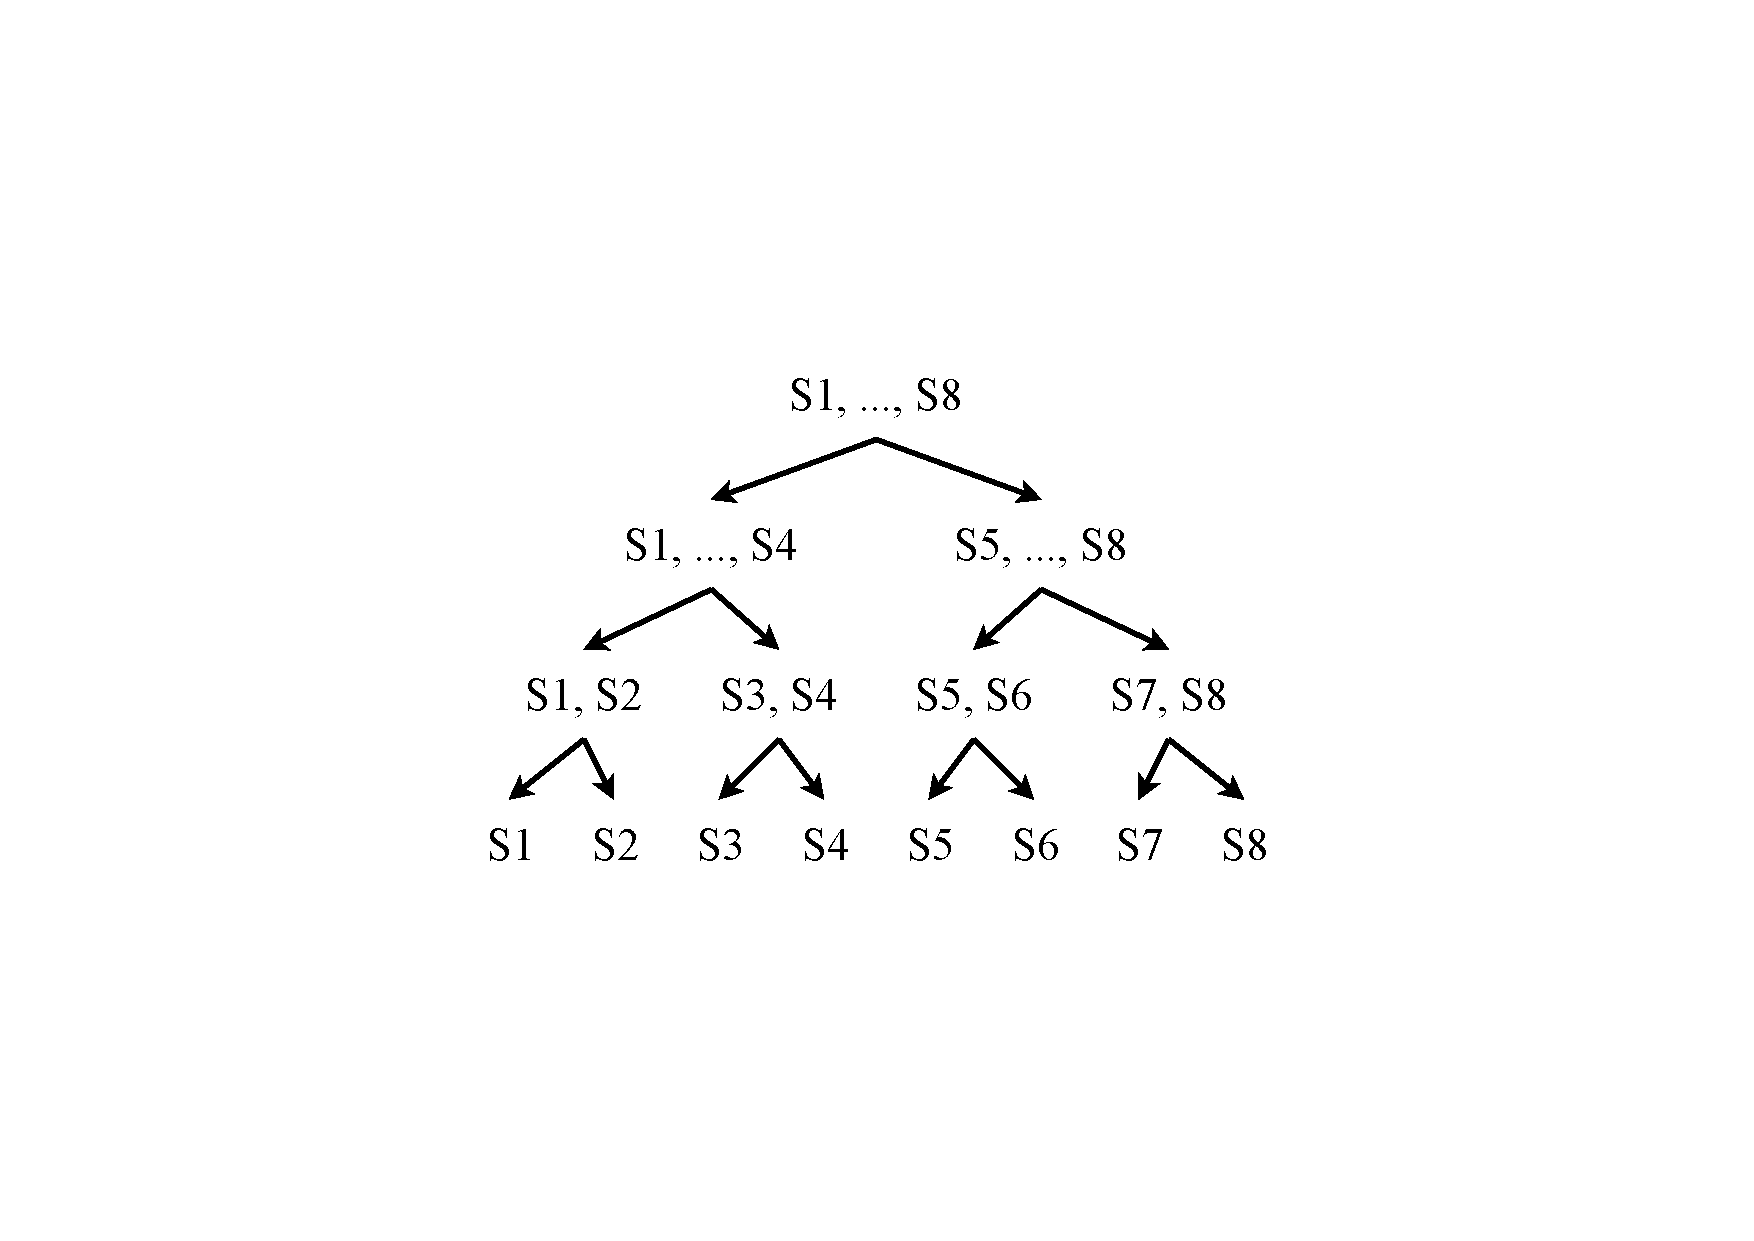
\includegraphics[scale=.45, clip,  trim=230 182 230 180]{img/arte/graphs-wavelet-tree.pdf}
    		
    		(a)
    	\end{minipage}
    	\begin{minipage}{0.5\textwidth}
    		\centering
    		%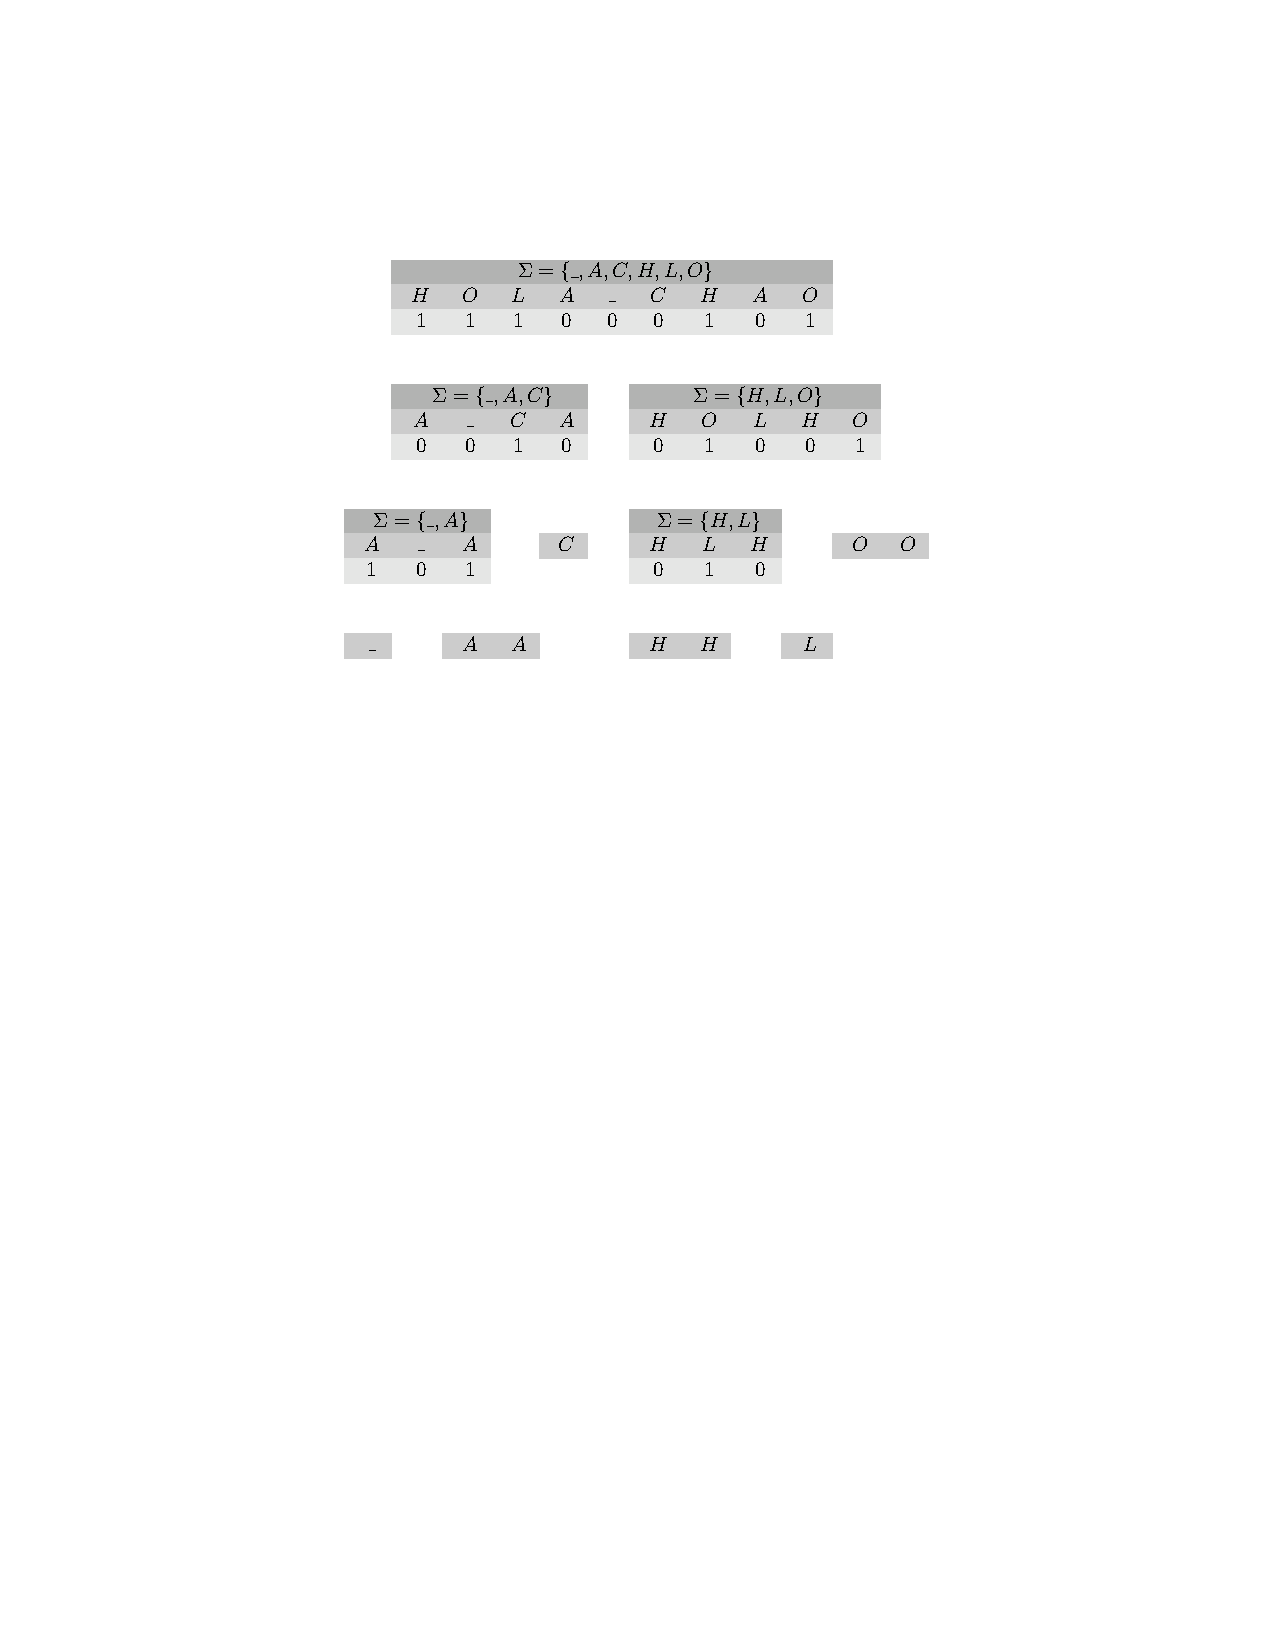
\includegraphics[scale=.8, clip, trim=150 475 150 120]{img/arte/wavelet-tree2.pdf}
    		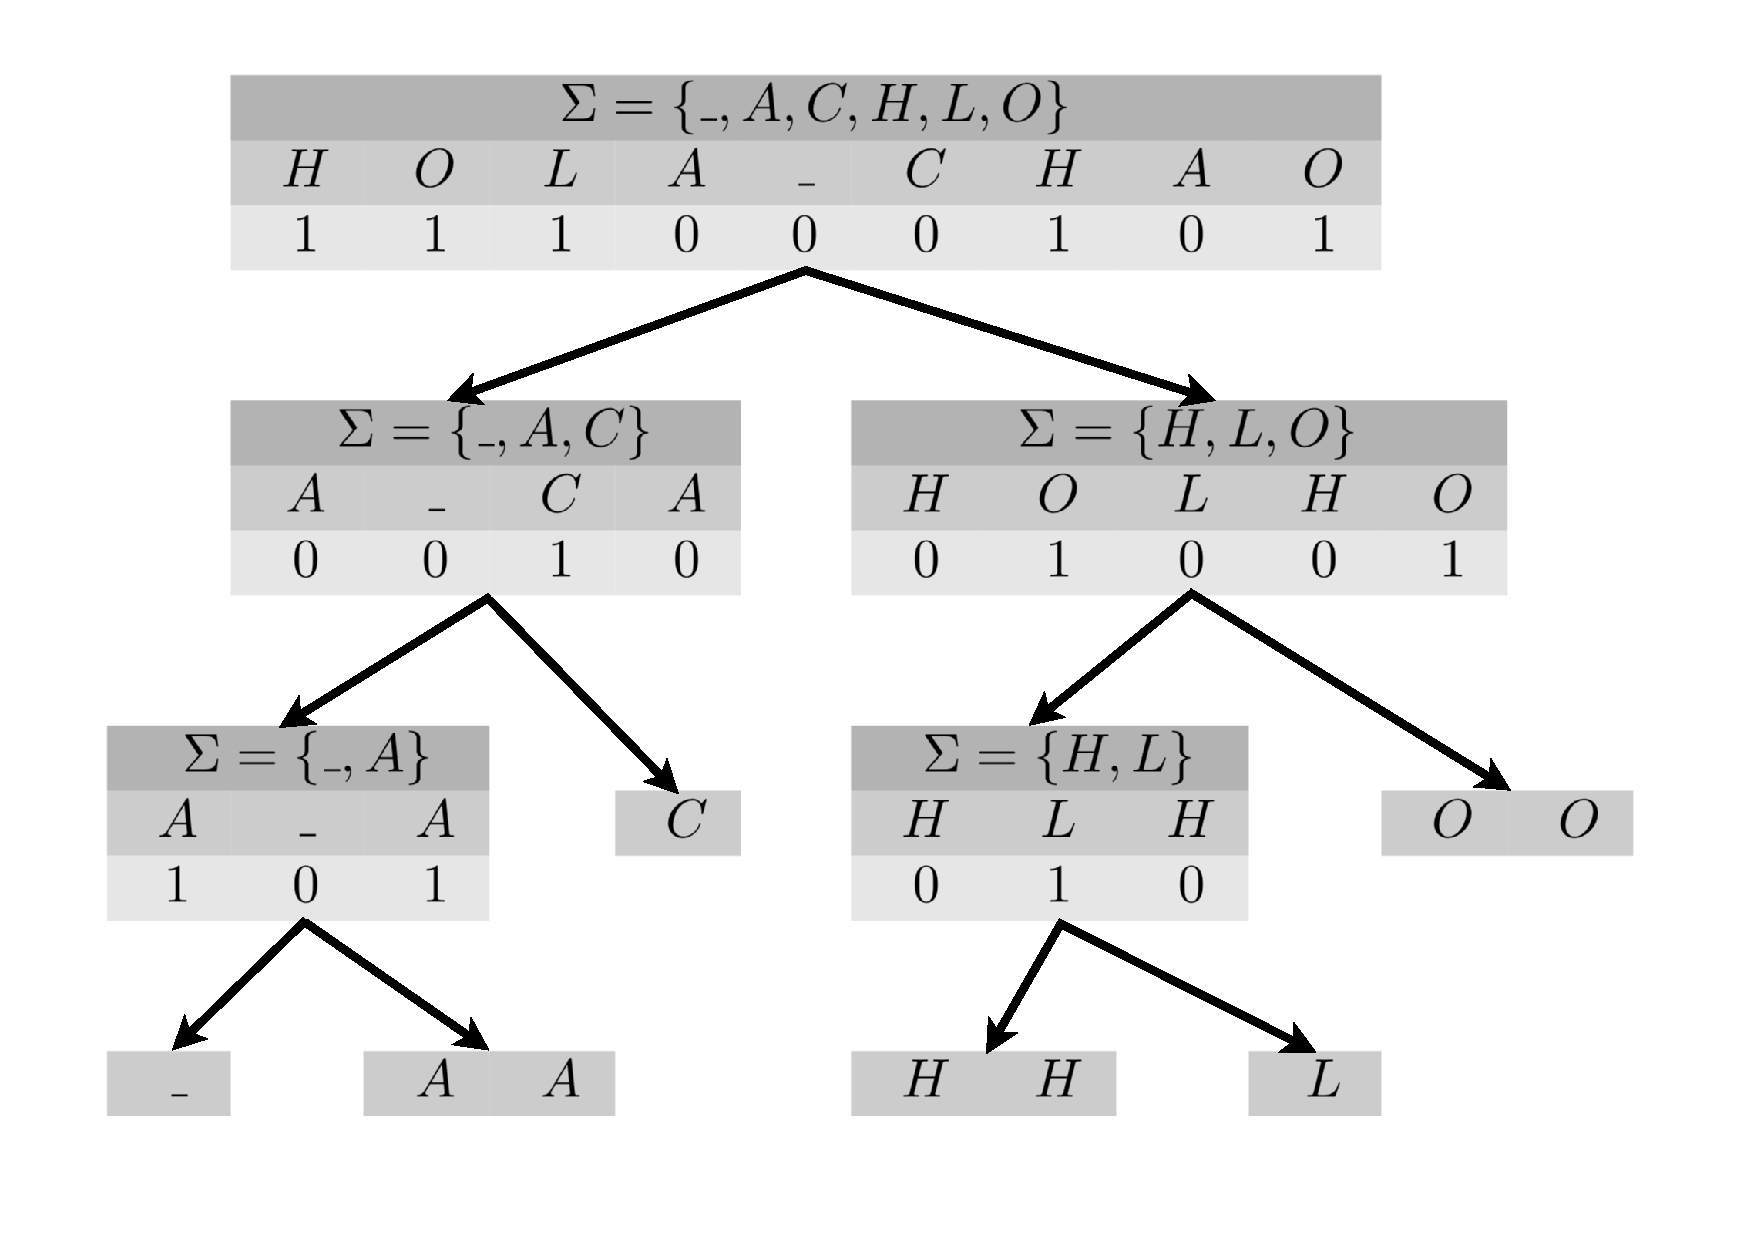
\includegraphics[scale=.3, clip, trim=0 0 0 0]{img/arte/graphs-wavelet-tree2.pdf}

    		(b)
    	\end{minipage}

    \caption{Ejemplos de wavelet-tree. (a) Ejemplo básico de subdivisión de secuencia ordenada. (b) Ejemplo práctico con alfabetos y bitmaps por nodo.}
    \label{fig:wavelet-tree}
\end{figure}

%    		\begin{tabular}{cccccccccccccc}
%	& & \multicolumn{9}{c}{\cellcolor{G} $\Sigma = \{\_,A, C, H, L, O\}$} & & & \\
%	& & \cellcolor{LG} $H$ & \cellcolor{LG} $O$ & \cellcolor{LG} $L$ & \cellcolor{LG} $A$ & \cellcolor{LG} $\_$ & \cellcolor{LG} $C$ & \cellcolor{LG} $H$ & \cellcolor{LG} $A$ & \cellcolor{LG} $O$ & & & \\
%	& & \cellcolor{LLG} $1$ & \cellcolor{LLG} $1$ & \cellcolor{LLG} $1$ & \cellcolor{LLG} $0$ & \cellcolor{LLG} $0$ & \cellcolor{LLG} $0$ & \cellcolor{LLG} $1$ & \cellcolor{LLG} $0$ & \cellcolor{LLG} $1$ & & & \\
%	\\
%	\\
%	 & & \multicolumn{4}{c}{\cellcolor{G} $\Sigma = \{\_,A, C\}$} & & \multicolumn{5}{c}{\cellcolor{G} $\Sigma = \{H, L, O\}$} & & \\
%	& & \cellcolor{LG} $A$ & \cellcolor{LG} $\_$ & \cellcolor{LG} $C$ & \cellcolor{LG} $A$ &  & \cellcolor{LG} $H$ & \cellcolor{LG} $O$ & \cellcolor{LG} $L$ & \cellcolor{LG} $H$ & \cellcolor{LG} $O$ &  & \\
%	& & \cellcolor{LLG} 0 & \cellcolor{LLG} 0 & \cellcolor{LLG} 1 & \cellcolor{LLG} 0 &  & \cellcolor{LLG} 0 & \cellcolor{LLG} 1 & \cellcolor{LLG} 0 & \cellcolor{LLG} 0 & \cellcolor{LLG} 1 &  & \\
%	\\
%	\\
%	& \multicolumn{3}{c}{\cellcolor{G} $\Sigma = \{\_,A\}$} & & & &  \multicolumn{3}{c}{\cellcolor{G} $\Sigma = \{H, L\}$} & & & & \\
%	& \cellcolor{LG} $A$ & \cellcolor{LG} $\_$ & \cellcolor{LG} $A$ &  & \cellcolor{LG} $C$	 &  & \cellcolor{LG} $H$ & \cellcolor{LG} $L$ & \cellcolor{LG} $H$ &  & \cellcolor{LG} $O$ & \cellcolor{LG} $O$ & \\
%	& \cellcolor{LLG} 1 & \cellcolor{LLG} 0 & \cellcolor{LLG} 1 &  &  &  & \cellcolor{LLG} 0 & \cellcolor{LLG} 1 & \cellcolor{LLG} 0 &  &  &  &  \\
%	\\
%	\\
%	& \cellcolor{LG} $\_$ & & \cellcolor{LG} $A$ & \cellcolor{LG} $A$ & & & \cellcolor{LG} $H$ & \cellcolor{LG} $H$ & & \cellcolor{LG} $L$ & & & \\ 
%\end{tabular}

Se construye de la siguiente manera. Dada una secuencia $S$ de largo $n = |S|$, donde $S[i] \in \Sigma$ y $\sigma = |\Sigma|$, se tiene: La raíz del árbol consiste en un bitmap $B$ donde $B[i] = 0$ si $S[i] \in [0, \frac{\sigma}{2}]$ y $B[i] = 1$ si $S[i] \in [\frac{\sigma}{2} + 1, \sigma]$. El siguiente nivel del árbol se construye basado en los símbolos asociados al nodo por el bitmap $B$ padre. Para $B[i] = 0$, se crea el bitmap hijo de la izquierda, y el alfabeto asociado a esos símbolos nuevamente se divide en dos, asignando valor a dicho bitmap siguiendo el mismo procedimiento descrito anteriormente. De manera similar, para $B[i] = 1$ se crea el bitmap derecho y se sidue el mismo procedimiento. Esto se repite por cada nodo hasta llegar a símbolos únicos en cada nodo terminal. Se requiere guardar los punteros a cada nodo hijo izquierdo y derecho, con los que se permite la navegación por el árbol.

Mejorando la propuesta de wavelet tree \cite{grossi2003high}, Claude, Navarro y Ordóñez \cite{claude2015wavelet} proponen una nueva estructura llamada \textbf{wavelet matrix}. Primero crean una versión de wavelet tree sin punteros, reemplazando cada bitmap por nodo por solo un bitmap por nivel, y contando la cantidad de ceros pueden determinar las subdivisiones pertinentes en cada nivel. 

Luego, para crear la wavelet matrix, liberan a la estructura de la suposición que los hijos de un nodo $v$ deben ir alineados. Esto les permite diseñar un mecanismo de clasificación mas sencillo entre un nivel y otro: todos los ceros pasan a la izquierda y todos los unos a la derecha. Por cada nivel, guardan en un entero $z_{\ell}$ la cantidad de ceros del nivel $\ell$. En la Figura~\ref{fig:wavelet-matrix} se presentan en (a) un wavelet tree de ejemplo, en (b) su correspondiente wavelet tree sin punteros, y en (c) su wavelet matrix, donde las líneas verticales representan el valor de $z_{\ell}$ para cada nivel.

\begin{figure}%[b]
    	\centering
    	\begin{minipage}{0.3\textwidth}
    		\centering
    		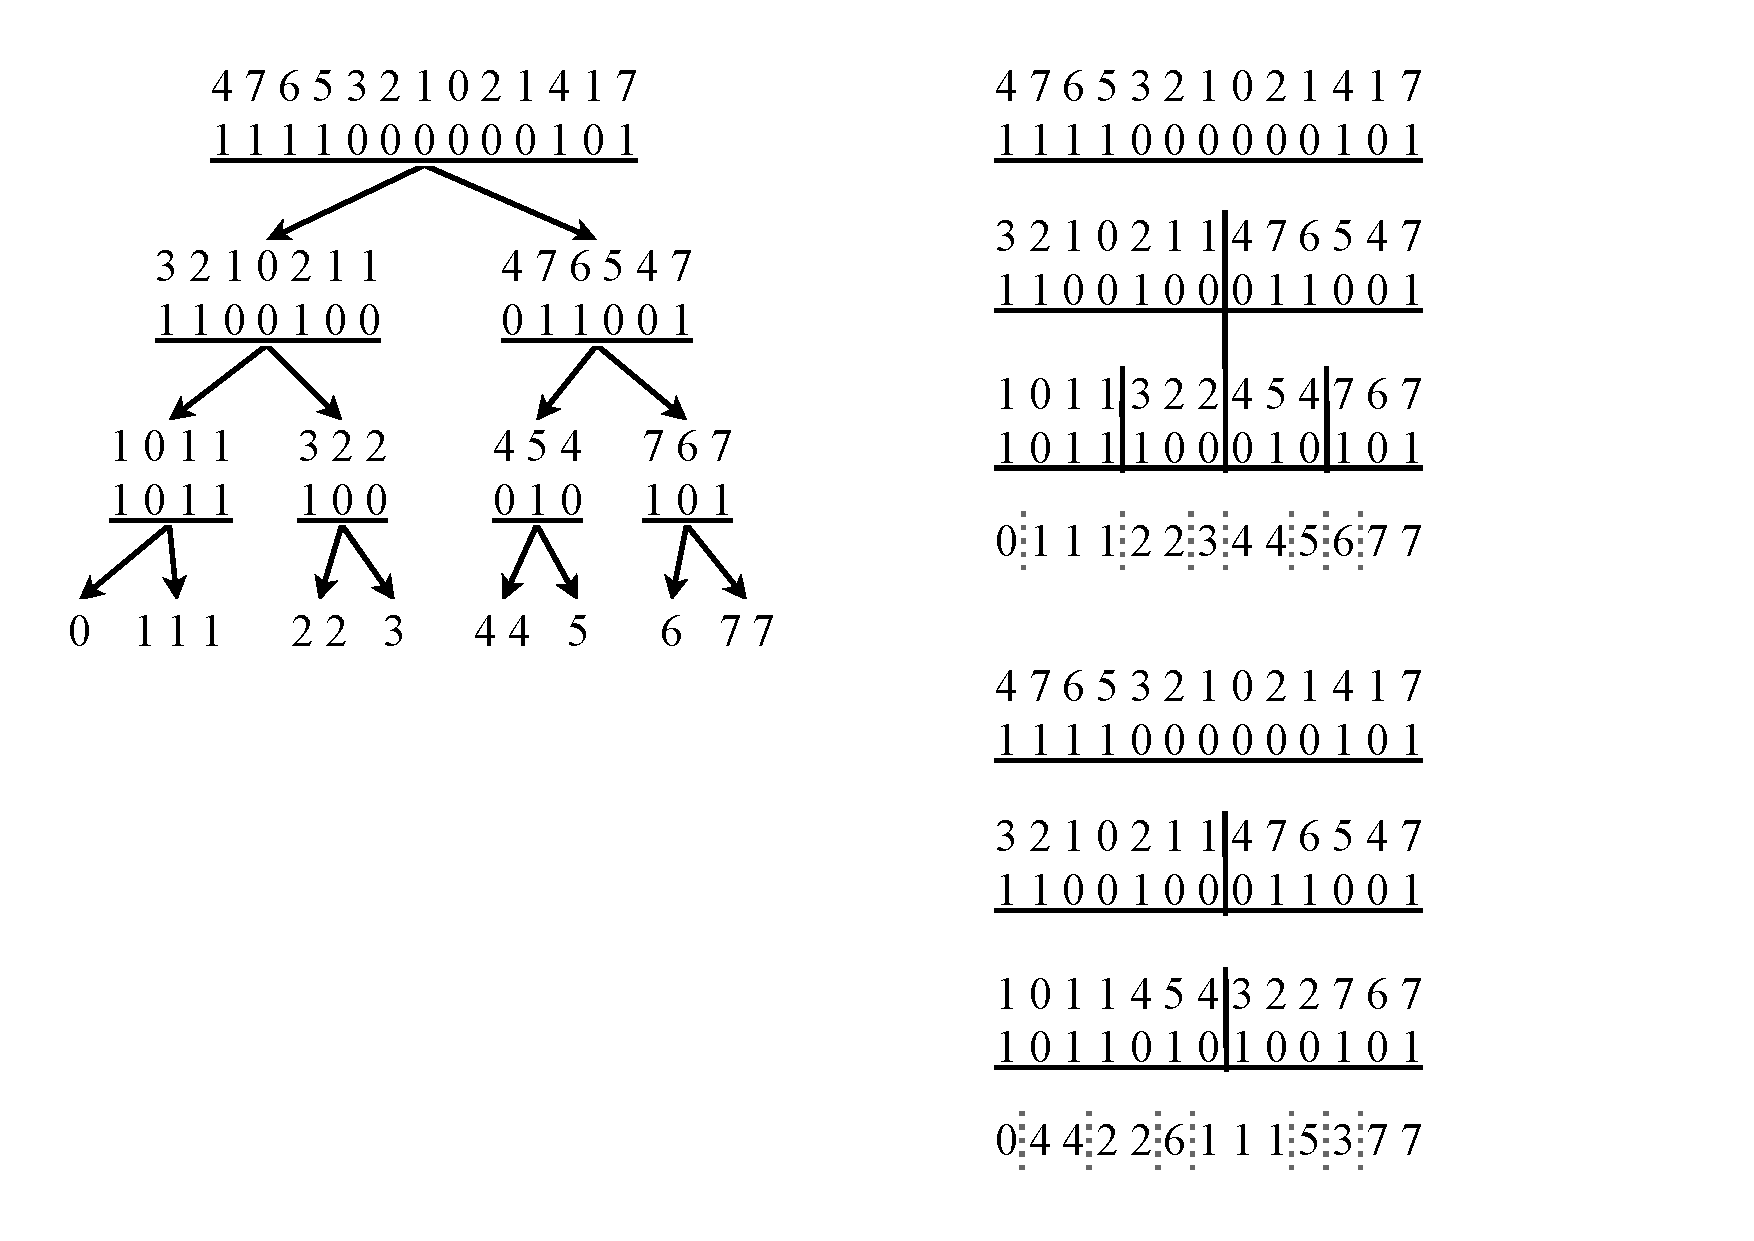
\includegraphics[scale=.4, clip,  trim=30 280 440 30]{img/arte/graphs-wavelet-matrix.pdf}
    		
    		(a)
    	\end{minipage}
    	\begin{minipage}{0.3\textwidth}
    		\centering
    		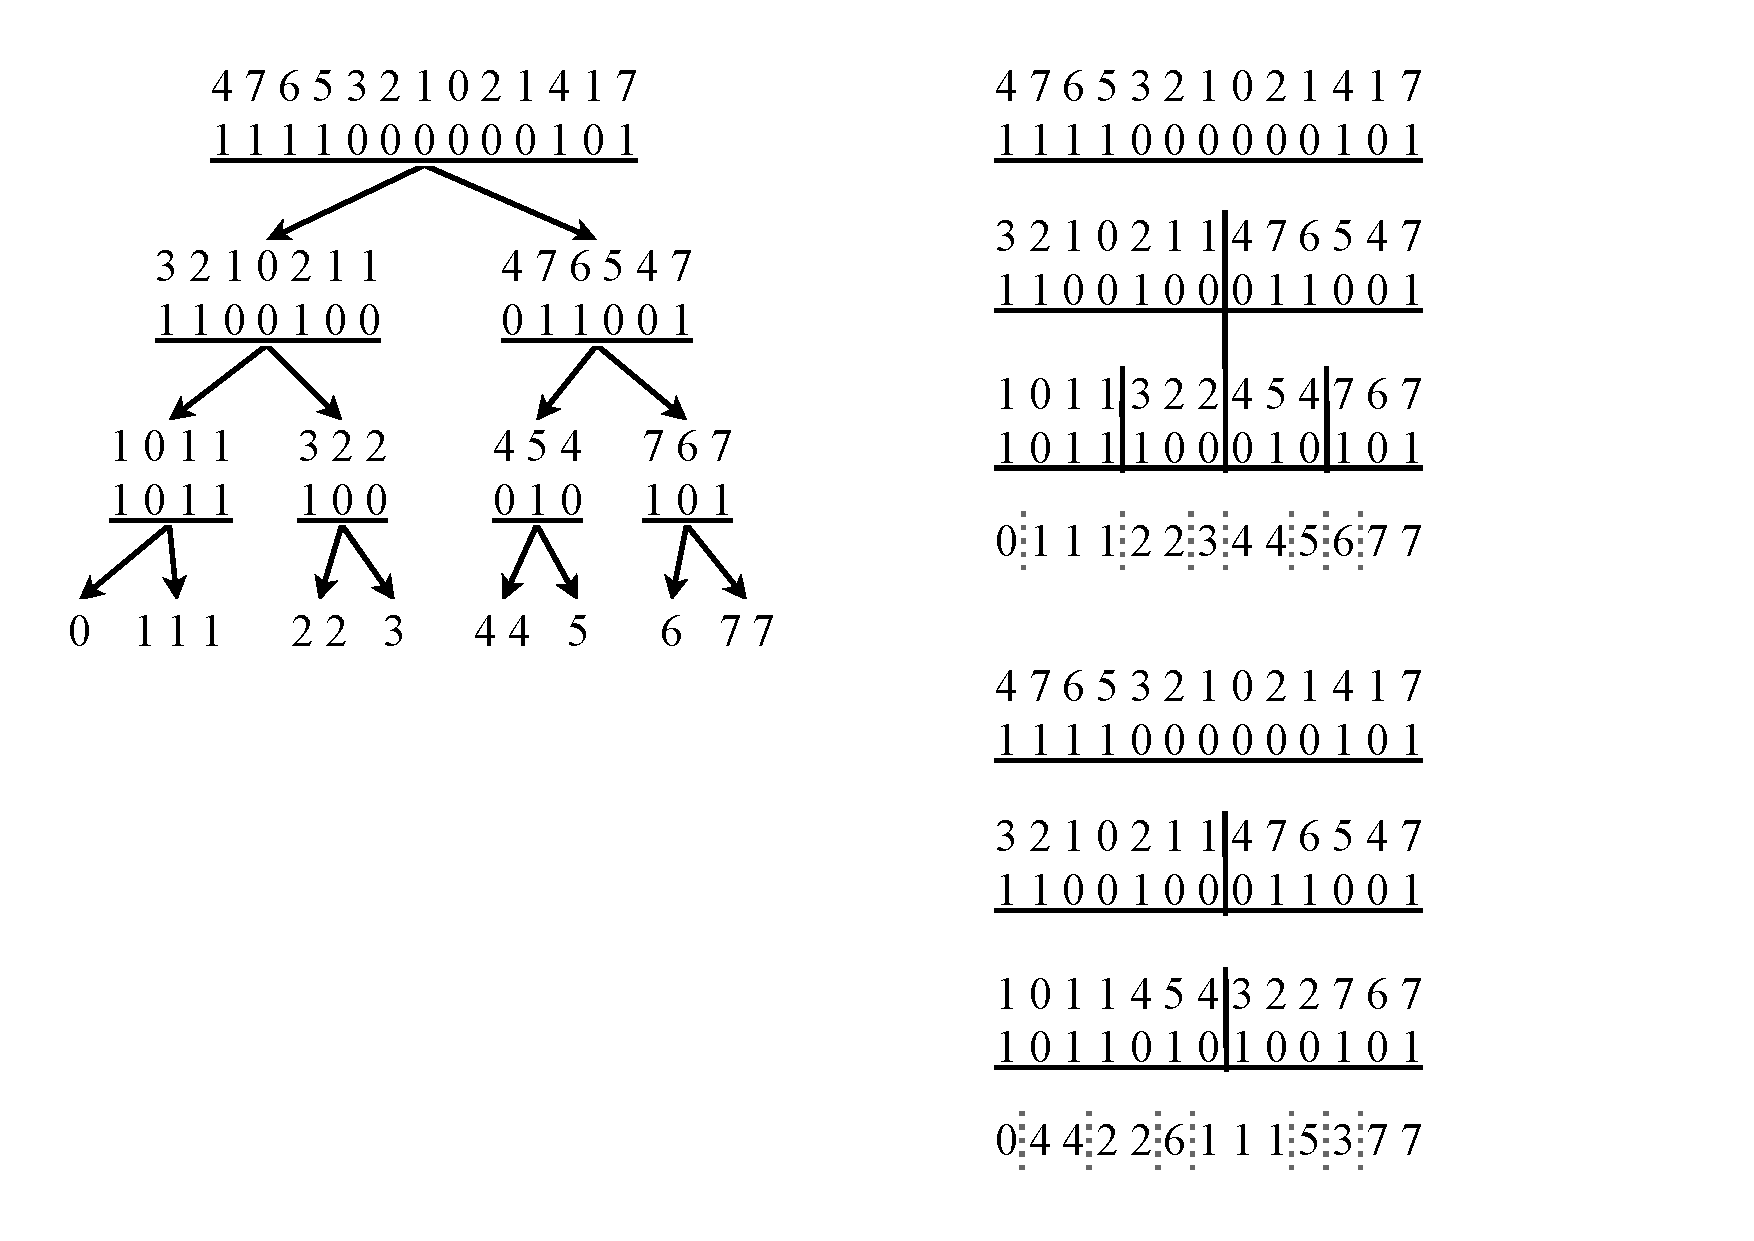
\includegraphics[scale=.45, clip, trim=470 320 170 30]{img/arte/graphs-wavelet-matrix.pdf}

    		(b)
    	\end{minipage}
    	\begin{minipage}{0.3\textwidth}
    		\centering
    		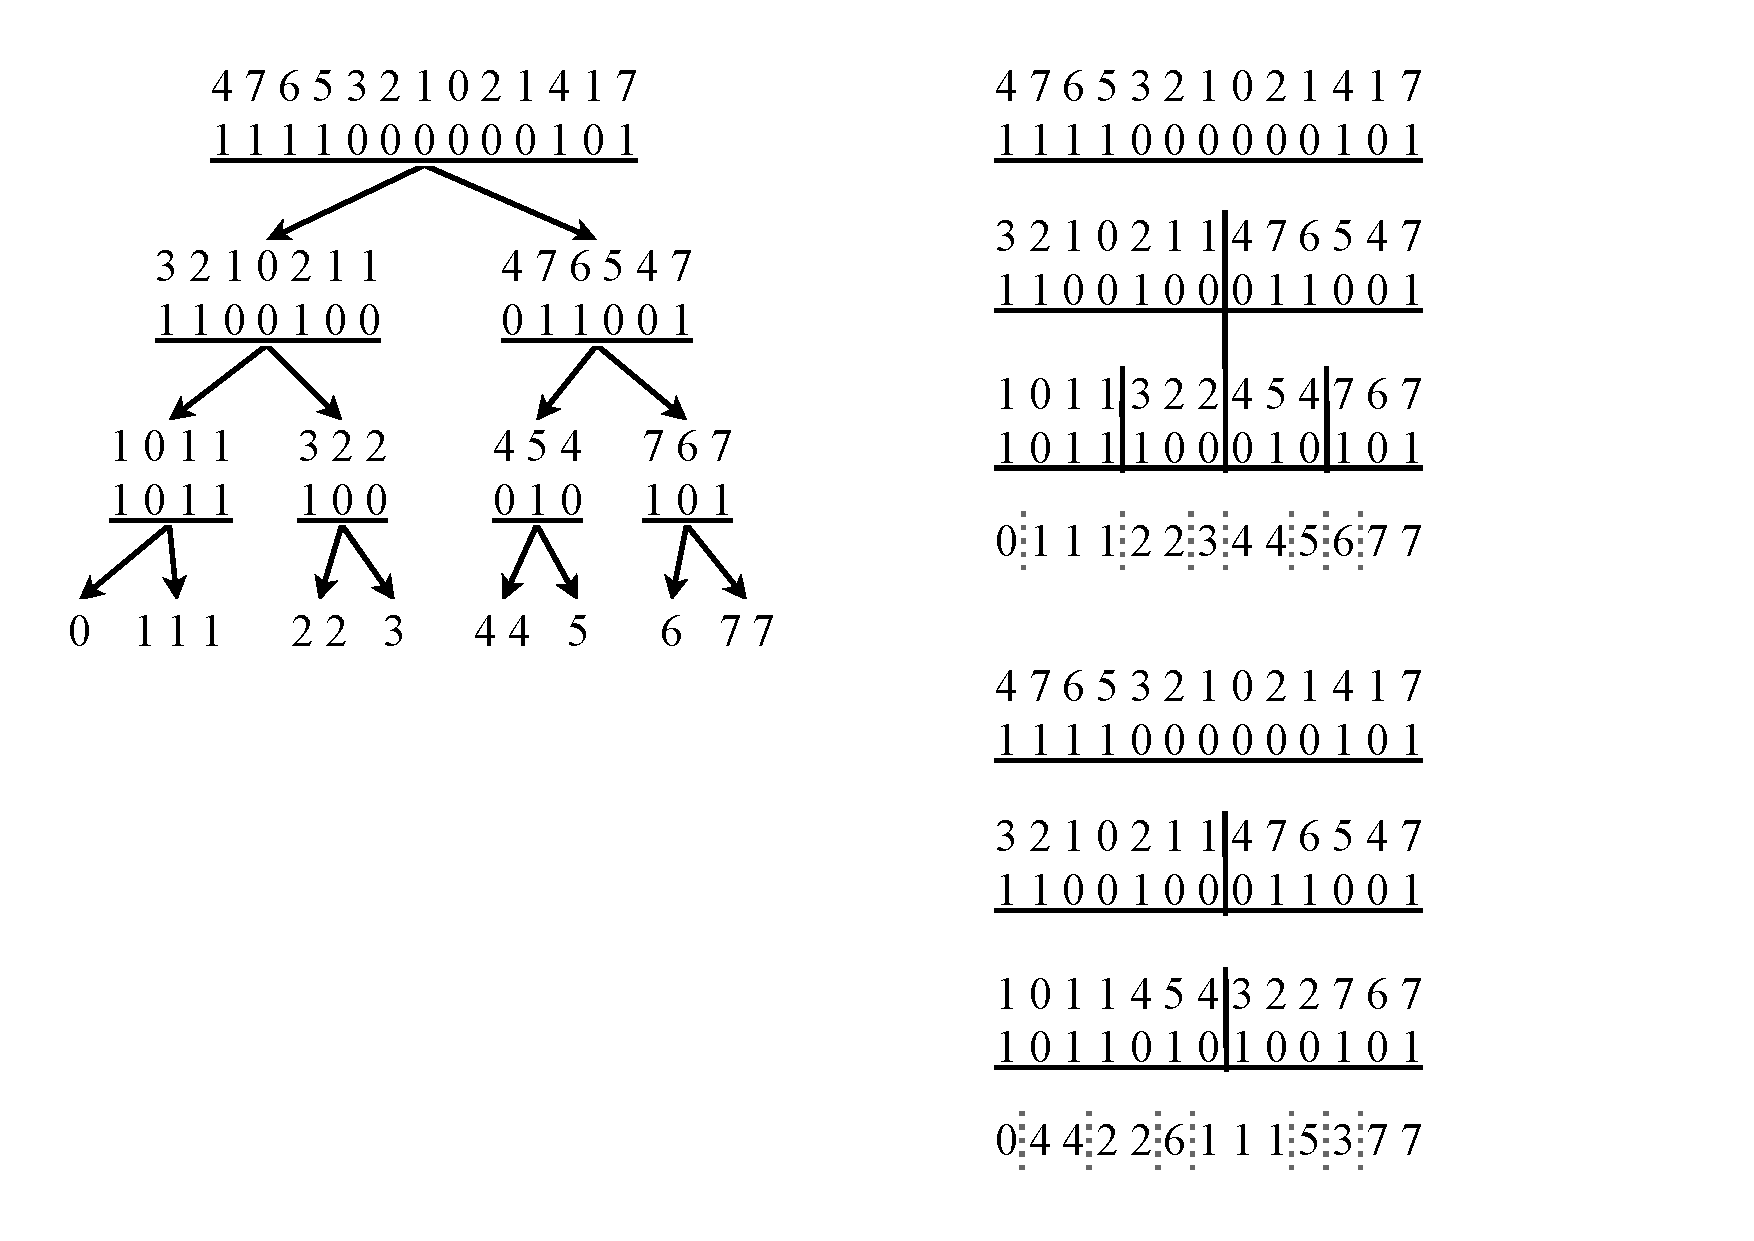
\includegraphics[scale=.45, clip, trim=470 33 170 317]{img/arte/graphs-wavelet-matrix.pdf}

    		(c)
    	\end{minipage}

    \caption{Ejemplos para wavelet-matrix. (a) Un wavelet tree. (b) El mismo wavelet tree sin punteros. (c) La wavelet matrix correpondiente.}
    \label{fig:wavelet-matrix}
\end{figure}


También prueban otras alternativas de representación, como usar Huffman \cite{huffman1952method} tanto para la representación sin punteros del wavelet-tree como para la wavelet matrix. Su resultado apunta a la superioridad tanto en tiempo como espacio en disco de wavelet matrix sobre wavelet-tree, lo que se tendrá en consideración a la hora de evaluarlos como alternativas de compresión.

\subsection{SDSL - Succinct Data Structure Library}
Gog, Beller, Moffat y Petri \cite{gbmp2014sea} desarrollan la librería \texttt{SDSL}\footnote{\url{https://github.com/simongog/sdsl-lite}} (Succinct Data Structure Library), desarrollada en \texttt{C++11} y registrada bajo \texttt{GPLv3}, donde se pueden utilizar las estructuras planteadas en las secciones anteriores, entre muchas otras más.



\section{Detección de cliques maximales} \label{sec:Cliques}
La detección de cliques maximales en un grafo es un problema NP-Hard \cite{karp1972reducibility}. Se han buscado una solución desde varios enfonques \cite{bron1973algorithm, eblen2012maximum, hendrix2010theoretical, bomze1999maximum, eppstein2010listing, eppstein2011listing}. siendo la más destacada para este trabajo lo propuesto por Eppstein y Strash \cite{eppstein2011listing}, basado en el trabajo de Eppstein, Löffler y Strash \cite{eppstein2010listing}, enfocado a grafos poco densos.

Eppstein et al. \cite{eppstein2010listing} presentan una modificación al algoritmo de Bron–Kerbosch \cite{bron1973algorithm}, que permite encontrar los cliques maximales de un grafo poco denso, con $n$ nodos y \textit{degeneracy} $d$, en un tiempo $O(dn3^{d/3})$.

Antes de detallar el funcionamiento de los algoritmos, primero es necesario definir lo siguiente: Sea un grafo $G = (V, E)$, con $n$ vértices y $m$ aristas. Para un vértice $v$ se define $\Gamma(v)$ como el set $\{w | (v, w) \in E\}$, llamado la \textit{vecindad} de $v$, y similarmente para un subset $W \subset V$ se define $\Gamma(W)$ como el set $\cap_{w \in W} \Gamma(w)$, llamado la \textit{vecindad común} de todos los vértices en $W$.

El algoritmo de Bron–Kerbosch \cite{bron1973algorithm} es un algoritmo \textit{backtracking} recursivo, sencillo y muy usado para encontrar el listado de cliques maximales de un grafo. Una llamada recursiva entrega tres sets separados de nodos: $R$, $P$, y $X$. $R$ es un clique (posiblemente no maximal), y $P \cup X = \Gamma(R)$ son todos los vértices adyacentes a cada vértice en $R$. Los nodos en $P$ son aquellos que serán considerados para añadirse a $R$, y los pertenecientes a $X$ deben ser excluidos del clique. El algoritmo elige un candidato en $v \in P$ para añadirlo al clique $R$, realiza una llamada recursiva con $v$ ya movido de $P$ a $R$, y con $X$ restringido a los vecinos de $v$. Cuando la llamada recursiva retorna, $v$ se mueve a $X$ para evitar trabajo redundante. Cuando la recursión llega al punto donde $P$ y $X$ están vacíos, $R$ es reportado como un clique maximal. Para obtener todos los cliques maximales, se debe iniciar la recursión con $P$ igual a todos los nodos del grafo, y $R$ con $X$ vacíos.

También describen la heurística llamada \textit{pivoting}, que limita la cantidad de llamadas recursivas realizadas por el algoritmo. Para cualquier nodo $u \in P \cup X$, llamado \textit{pivot}, cualquier clique maximal debe contener algún nodo no vecino de $u$, incluido si mismo. Por tanto, se retrasa que los vértices en $P \cap \Gamma(u)$ sean añadidos al clique, beneficiando realizar menos llamadas recursivas. Tomita et al. \cite{tomita2006worst} demuestran que eligiendo el \textit{pivot} $u$ para maximizar $|P \cap \Gamma(u)|$, se garantiza un orden de tiempo $O(3^{n/3})$.

Eppstein et al. \cite{eppstein2010listing} prueban que el orden de procesamiento de los vértices de $G$ por el algoritmo de Bron–Kerbosch también es importante. Lo primero que hacen es un ordenamiento por \textit{degeneracy} de los nodos del grafo, y en ese orden hacen las llamadas recursivas del algoritmo, usando la regla de \textit{pivot} de Tomita. En la Figura~\ref{fig:degenOrder} se ilustra un ejemplo de ordenamiento por \textit{degeneracy}. Gracias a esto, garantizan que su algoritmo propuesto logra listar todos los cliques maximales en un tiempo $O(dn3^{d/3})$.

arte-degenOrder

%Luego, Eppstein y Strash \cite{eppstein2011listing} implementan una variante al algoritmo propuesto, donde 
